\documentclass{article}
\usepackage{graphicx} % Required for inserting images
\usepackage[utf8]{inputenc}
\usepackage[vietnamese]{babel}
\usepackage{indentfirst}
\usepackage{biblatex}
\usepackage{tikz}
\usetikzlibrary{calc}
\usepackage{listings}
\usepackage{courier}
\usepackage{soul}
\usepackage[utf8]{inputenc}
\usepackage[a4paper, margin=0.4in]{geometry}
\newcommand\HRule{\rule{\textwidth}{1pt}}
\usepackage[colorlinks=true, urlcolor=blue]{hyperref}
\usepackage{enumitem}
\usepackage{xcolor}

\begin{document}
\begin{titlepage}

\begin{center}

TRƯỜNG ĐẠI HỌC KHOA HỌC TỰ NHIÊN\\
\textbf{KHOA CÔNG NGHỆ THÔNG TIN}\\[2cm]

{ \large \bfseries Nguyễn Đức Tài - Phạm Hoàng Hải Đăng\\ Lê Hồng Thạch - Trần Đình Tấn Phát\\ Phan Nguyễn Gia Huy - Nguyễn Đỗ Bảo Kiên\\[2cm] } 


{ \large \bfseries ĐỒ ÁN MÔN GIỚI THIỆU TRÍ TUỆ NHÂN TẠO \\[3cm]} 


\large GIỚI THIỆU CHƯƠNG TRÌNH TỰ ĐỘNG PHÁT HIỆN BIỂN SỐ XE\\

\large CHƯƠNG TRÌNH CHÍNH QUY\\

\begin{tikzpicture}[remember picture, overlay]
  \draw[line width = 2pt] ($(current page.north west) + (1cm,-1cm)$) rectangle ($(current page.south east) + (-2cm,1cm)$);
\end{tikzpicture}

\vfill
Tp. Hồ Chí Minh, tháng 11/2024

\end{center}

\pagebreak
\end{titlepage}
\maketitle
%phần 1
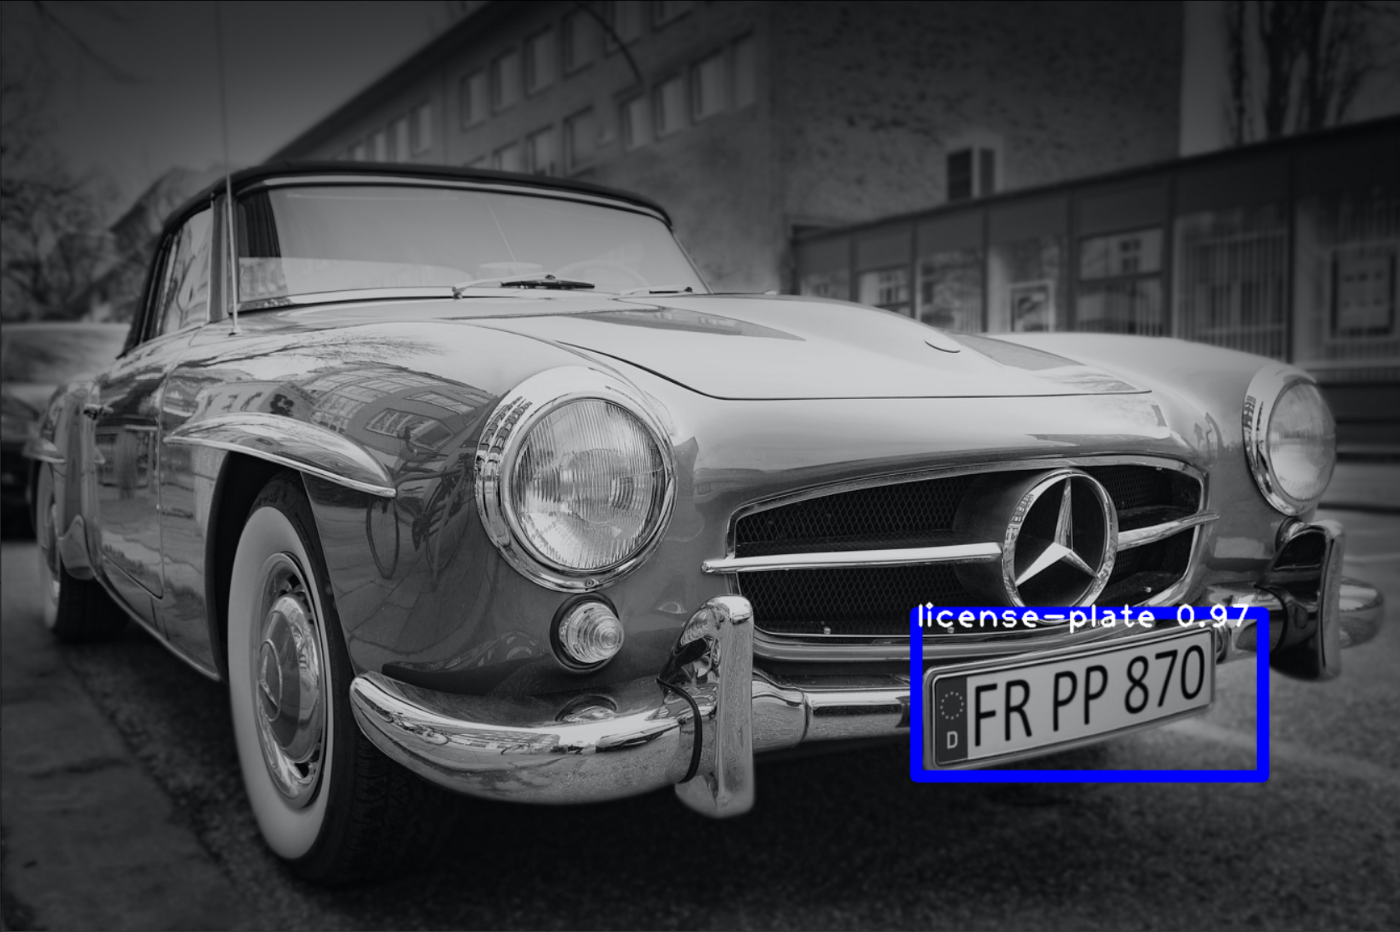
\includegraphics[width=10cm]{img/img1/Notebook1.png}

\tableofcontents


\textbf{ĐÁNH GIÁ THÀNH VIÊN}:
\begin{itemize}
    \item Nguyễn Đức Tài: nhiệt tình, hoạt bát. 
    \item Phạm Hoàng Hải Đăng: chăm chỉ, chịu khó.
    \item Lê Hồng Thạch: nhiệt tình, chịu khó.
    \item Trần Đình Tấn Phát: năng nổ, hoạt bát.
    \item Phan Nguyễn Gia Huy: cần cù, chăm chỉ.
    \item Nguyễn Đỗ Bảo Kiên: hòa đồng, chăm chỉ.
\end{itemize}


\textbf{ĐÁNH GIÁ MỨC ĐỘ HOÀN THÀNH CHO TỪNG YÊU CẦU}:

\begin{itemize}
    \item Source code: xong 
    \item slide: xong
    \item Video: xong 
    \item Report:xong
\end{itemize}

\setlength{\parindent}{1cm}
\section{MỤC GIỚI THIỆU}
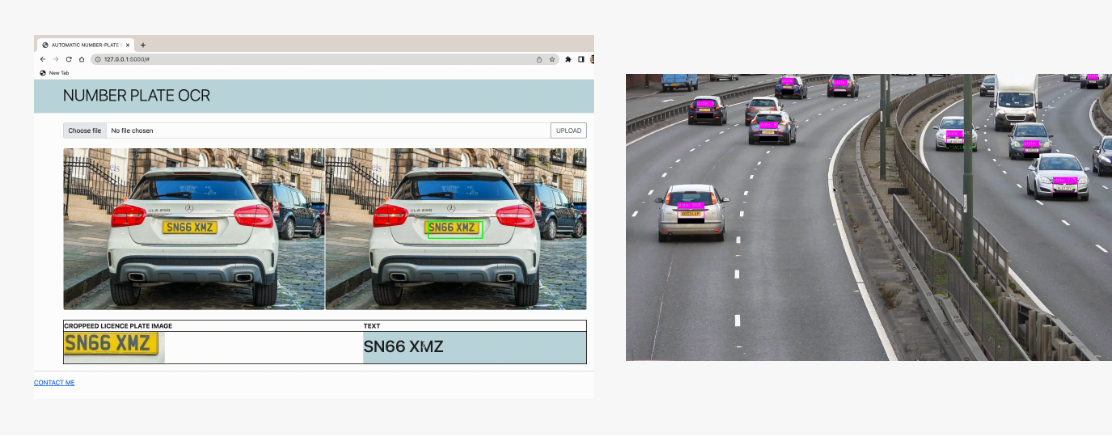
\includegraphics[width= 10cm]{img/img1/Screenshot 2024-11-20 165252.png}

Trong thời đại ngày nay, bảo mật đã trở thành một trong những mối quan tâm lớn nhất của bất kỳ tổ chức nào và việc tự động hóa bảo mật như vậy là điều cần thiết. Tuy nhiên, nhiều giải pháp hiện tại vẫn chưa mạnh mẽ trong các tình huống thực tế, thường phụ thuộc vào nhiều ràng buộc. Trong dự án sau, chúng ta sẽ tìm hiểu cách nhận dạng biển số xe bằng ngôn ngữ lập trình Python.

Chúng ta sẽ sử dụng OpenCV cho dự án này để nhận dạng biển số xe và python pytesseract để trích xuất các ký tự và chữ số từ biển số. Dự án này cũng sẽ trình bày một hệ thống ALPR mạnh mẽ và hiệu quả dựa trên trình phát
hiện đối tượng YOLO hiện đại. Chúng ta sẽ Ứng dụng web với chương trình Python tự động nhận dạng Biển số xe vào cuối bài viết này. Kết quả cho thấy mạng nơ-ron được đào tạo có thể thực hiện với độ chính xác cao gần 90-95 phần trăm trong việc nhận dạng biển số xe trong hình ảnh có độ phân giải thấp bằng hệ thống này.


\subsection{CÁC TRƯỜNG HỢP SỬ DỤNG}
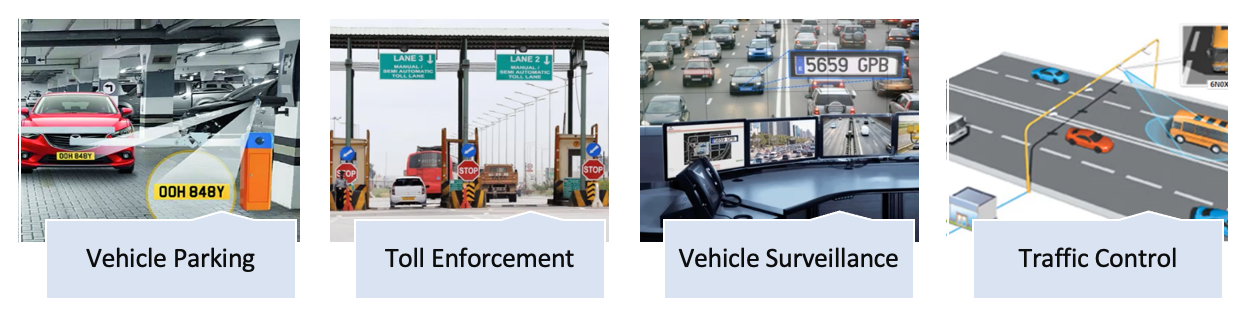
\includegraphics[width=10cm]{img/img1/Notebook2.png}

Phát hiện biển số xe là xác định phần của xe được dự đoán là biển số. Nhận dạng là xác định các giá trị tạo nên biển số xe. Phát hiện và nhận dạng biển số xe là công nghệ sử dụng thị giác máy tính để phát hiện và nhận dạng biển số xe từ hình ảnh đầu vào của xe. Công nghệ này được áp dụng trong nhiều lĩnh vực. Trên đường, công nghệ này được sử dụng để xác định những chiếc xe vi phạm luật giao thông. Trong an ninh, công nghệ này được sử dụng để chụp biển số xe của những phương tiện ra vào một số địa điểm nhất định. Trong bãi đỗ xe, công nghệ này được sử dụng để chụp biển số xe của những chiếc xe đang đỗ. Danh sách các ứng dụng của công nghệ này còn rất dài.

\subsection{CẤU TRÚC DỰ ÁN}

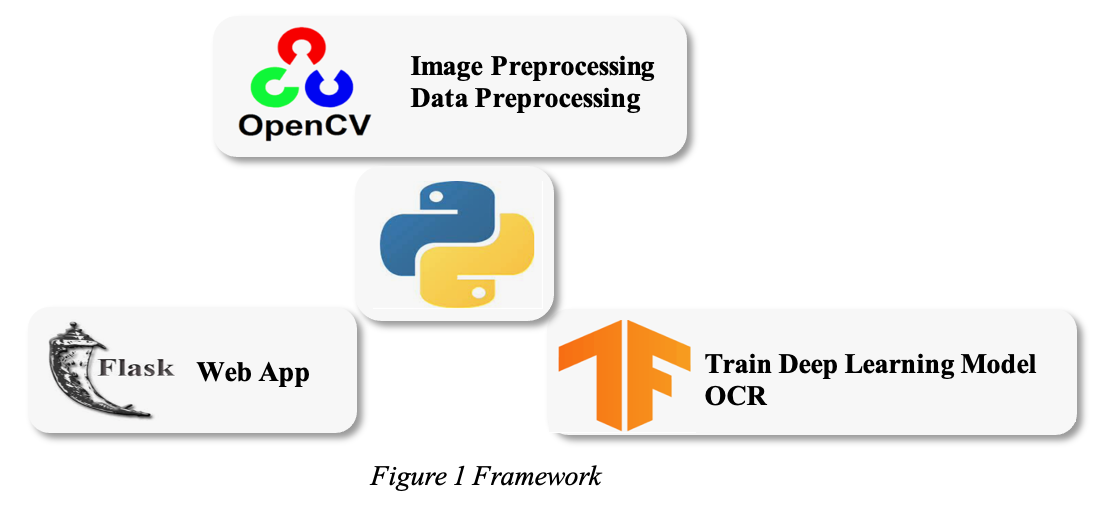
\includegraphics[width=10cm]{img/img1/Notebook3.png}\\
Trong cấu trúc bên dưới Hình 2, có sáu mô-đun. Gắn nhãn, Đào tạo, Lưu mô hình, OCR và Đường ống và API RESTful. Quy trình như sau.

Đầu tiên, chúng ta sẽ thu thập hình ảnh. Sau đó, chúng ta phải gắn nhãn hình ảnh để phát hiện đối tượng Biển số xe hoặc Biển số xe bằng Công cụ chú thích hình ảnh\href{https://github.com/Asikpalysik/Automatic-License-Plate-Detection/tree/main/labelImg-master}{\textcolor{blue}{Github}} , đây là phần mềm nguồn mở được phát triển bằng GUI python. 

Sau khi gắn nhãn hình ảnh, chúng ta sẽ xử lý dữ liệu trước, xây dựng và đào tạo mô hình phát hiện đối tượng học sâu (Inception Resnet V2) trong TensorFlow 2.

Sau khi hoàn tất quy trình đào tạo mô hình Phát hiện đối tượng, sau đó sử dụng mô hình này, chúng ta sẽ cắt ảnh có chứa biển số xe, còn được gọi là vùng quan tâm (ROI) và chuyển ROI tới API Nhận dạng ký tự quang học Tesseract trong Python (PyTesseract).

Cũng như trích xuất văn bản từ hình ảnh. Bây giờ, chúng ta sẽ tổng hợp tất cả lại với nhau và xây dựng mô hình Học sâu Đường ống. Trong mô-đun cuối cùng, chúng ta sẽ học cách tạo một dự án ứng dụng web bằng FLASK Python. Với điều đó, cuối cùng chúng ta đã sẵn sàng với Ứng dụng của mình.\\
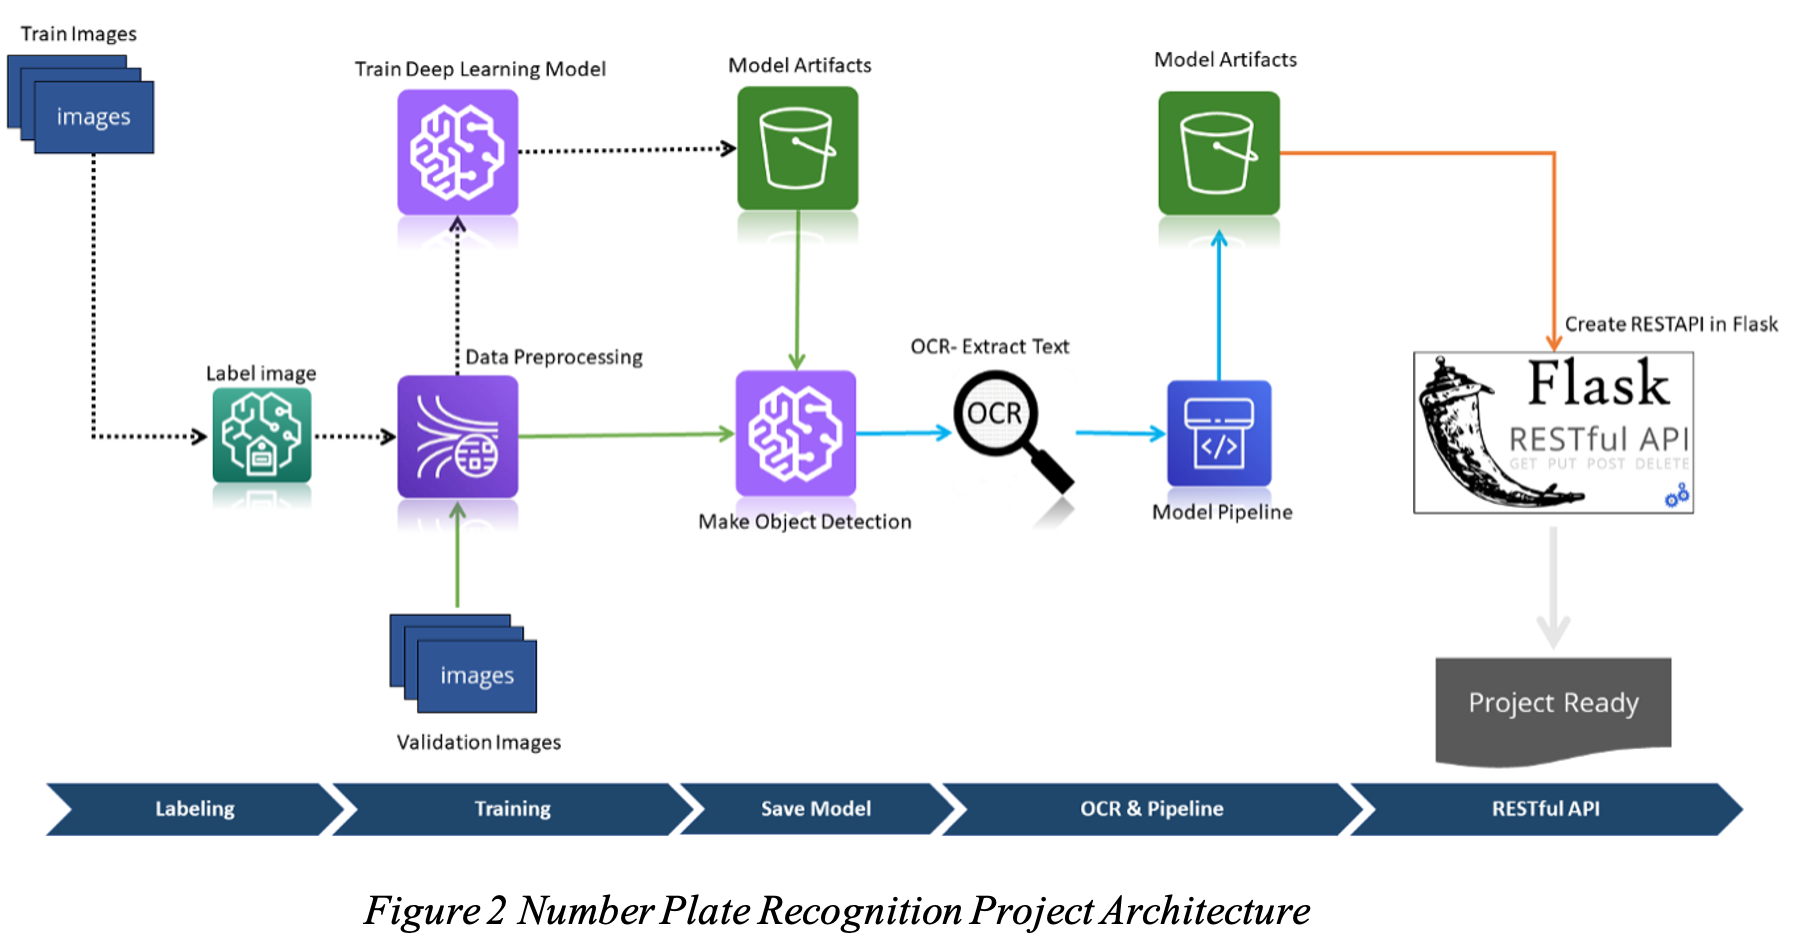
\includegraphics[width=10cm]{img/img1/Notebook4.png}\\

% phần 2
\section{PHÂN LOẠI}
\subsection{HIỂU VÀ THU THẬP DỮ LIỆU YÊU CẦU}
Để xây dựng nhận dạng biển số xe, chúng ta cần dữ liệu. Để làm được điều đó, chúng ta cần thu thập hình ảnh xe có biển số xe càng nhiều càng tốt.\href{https://github.com/Asikpalysik/Automatic-License-Plate-Detection/tree/main/images}{\textcolor{blue}{Đây}} là dữ liệu mẫu mà tôi đã sử dụng để xây dựng dự án này. Dưới đây bạn có thể thấy một số ví dụ Hình 3,4.\\
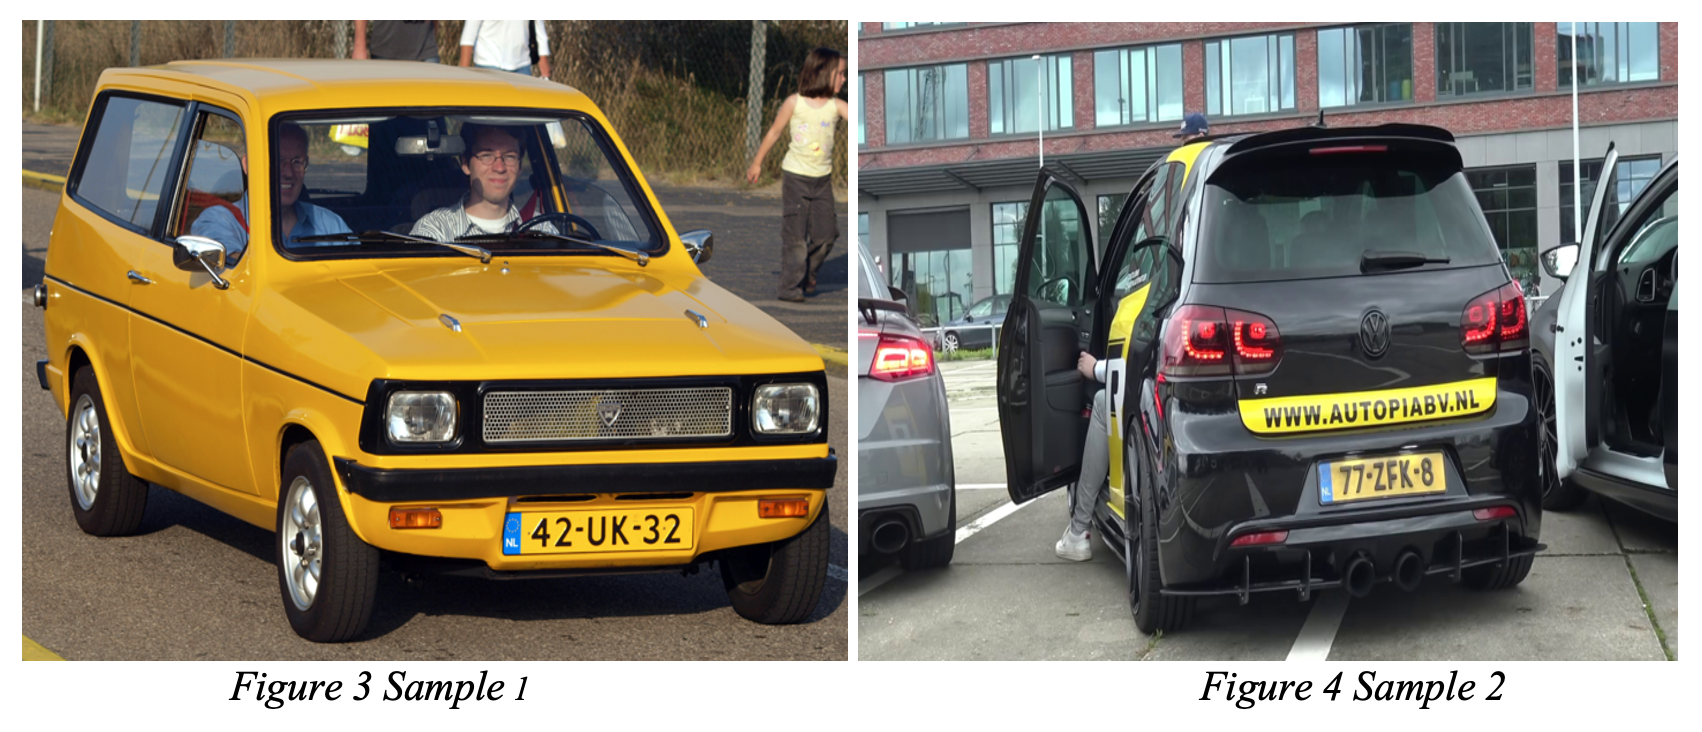
\includegraphics[width= 10cm]{img/img1/Notebook5.png}
\newpage
\subsection{PHÂN LOẠI ẢNH}

Đối với phân loại hình ảnh, tôi đã sử dụng công cụ chú thích hình ảnh LabelImg. Tải labelImg từ \href{https://github.com/Asikpalysik/Automatic-License-Plate-Detection/tree/main/labelImg-master}{\textcolor{blue}{GitHub}} và làm theo hướng dẫn để cài đặt gói. Sau đó mở GUI ra, đưa ra hướng dẫn và nhấp vào CreateRectBox và vẽ hộp hình chữ nhật như hình dưới đây và lưu đầu ra trong XML.

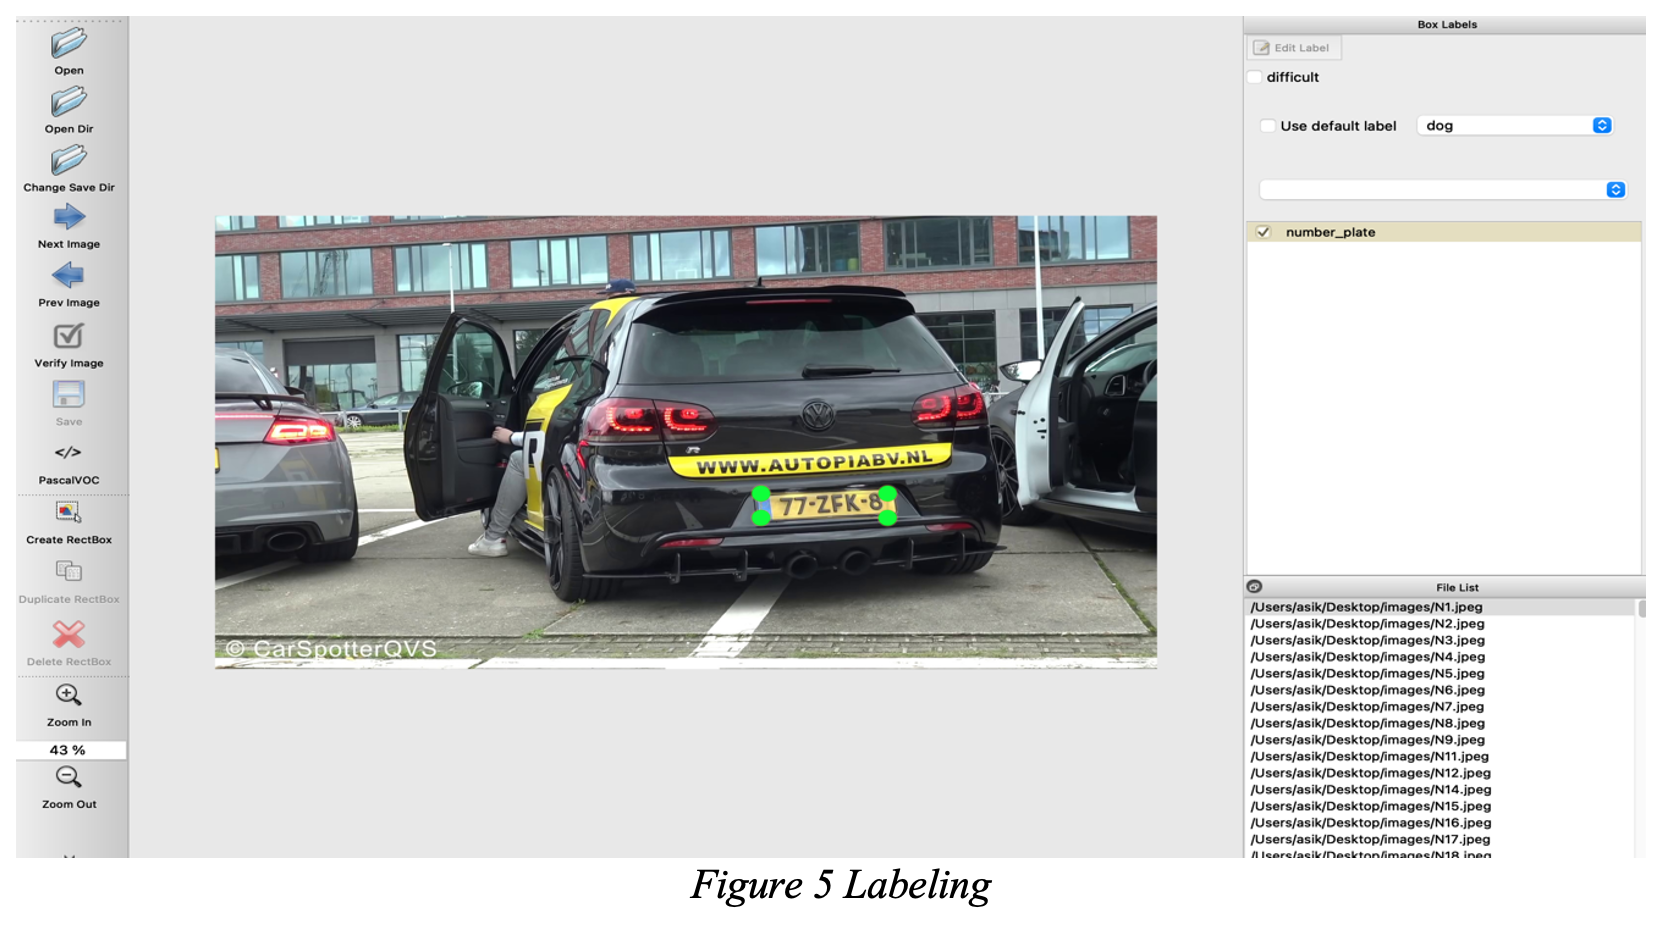
\includegraphics[width=10cm]{img/img1/Notebook6.png}\\

Đây là một quy trình thủ công và bạn cần thực hiện cho tất cả các hình ảnh. Hãy cẩn thận khi thực hiện dán nhãn vì quy trình dán nhãn có tác động trực tiếp đến độ chính xác của mô hình. \href{https://www.youtube.com/watch?v=XxslbNwcdaI}{\textcolor{blue}{Nhấp vào đây để xem video hướng dẫn}}. Trên Hình 5, bạn có thể tìm thấy cửa sổ chính.

\subsection{PHÂN TÍCH THÔNG TIN TỪ XML}


Ví dụ về tệp .xml của chúng tôi sẽ trông như bên dưới.\\

\begin{verbatim}
    <annotation>
    <folder>images</folder>
    <filename>N1.jpeg</filename>
    <path>/Users/asik/Desktop/ANPR/imagesN1.jpeg</path>
    <source>
        <database>Unknown</database>
    </source>
    <size>
        <width>1920</width>
        <height>1080</height>
        <depth>3</depth>
    </size>
    <segmented>0</segmented>
    <object>
        <name>number_plate</name>
        <pose>Unspecified</pose>
        <truncated>0</truncated>
        <difficult>0</difficult>
        <bndbox>
            <xmin>1093</xmin>
            <ymin>645</ymin>
            <xmax>1396</xmax>
            <ymax>727</ymax>
        </bndbox>
    </object>
</annotation>
\end{verbatim}

Sau khi hoàn tất quá trình gắn nhãn, giờ chúng ta cần xử lý trước dữ liệu. Vì đầu ra của nhãn là XML để sử dụng cho quá trình đào tạo nên chúng ta cần dữ liệu ở định dạng mảng. Đối với điều đó, chúng ta sẽ lấy thông tin hữu ích từ nhãn, đó là các điểm chéo của hộp hình chữ nhật hoặc hộp giới hạn tương ứng là xmin, ymin, xmax, ymax. Điều này có sẵn trong XML. Vì vậy, chúng ta cần trích xuất thông tin và lưu ở bất kỳ định dạng thuận tiện nào, ở đây tôi sẽ chuyển đổi thông tin giới hạn thành CSV và sau đó, tôi sẽ chuyển đổi thành một mảng bằng Pandas. Bây giờ chúng ta hãy xem cách phân tích cú pháp thông tin bằng Python.

\subsection{PHÂN TÍCH DỮ LIỆU TỪ XML VÀ CHUYỂN ĐỔI NÓ THÀNH CSV}

Trước tiên, hãy để tôi tải tất cả các thư viện mà tôi sẽ sử dụng trong dự án này cùng một lúc. Tôi cũng sẽ sử dụng thư viện python xml.etree để phân tích dữ liệu từ XML và cũng nhập pandas và glob. Sử dụng glob trước tiên hãy lấy tất cả các tệp XML được tạo ra trong quá trình gắn nhãn.\\
\begin{verbatim}
    print("hello world")
    --> hello world
\end{verbatim}

\textbf{\#} \textcolor{green}{2 cell phía dưới cài đặt các thư viện.}\\

!sudo apt install tesseract-ocr -y
-->
    Reading package lists... Done
Building dependency tree... Done
Reading state information... Done
The following additional packages will be installed:
  tesseract-ocr-eng tesseract-ocr-osd
The following NEW packages will be installed:
  tesseract-ocr tesseract-ocr-eng tesseract-ocr-osd
0 upgraded, 3 newly installed, 0 to remove and 24 not upgraded.
Need to get 4,816 kB of archives.
After this operation, 15.6 MB of additional disk space will be used.

Get:1\href{http://archive.ubuntu.com/ubuntu}{\textcolor{blue}{http://archive.ubuntu.com/ubuntu}} jammy/universe amd64 tesseract-ocr-eng all 1:4.00~git30-7274cfa-1.1 [1,591 kB]

Get:2 \href{http://archive.ubuntu.com/ubuntu}{\textcolor{blue}{http://archive.ubuntu.com/ubuntu}}jammy/universe amd64 tesseract-ocr-osd all 1:4.00~git30-7274cfa-1.1 [2,990 kB]

Get:3 \href{http://archive.ubuntu.com/ubuntu}{\textcolor{blue}{http://archive.ubuntu.com/ubuntu}} jammy/universe amd64 tesseract-ocr amd64 4.1.1-2.1build1 [236 kB]
\begin{verbatim}

Fetched 4,816 kB in 1s (8,783 kB/s)
debconf: unable to initialize frontend: Dialog
debconf: (No usable dialog-like program is installed, so the dialog based frontend cannot be used. at /usr/share/perl5/Debconf/FrontEnd/Dialog.pm line 78, <> line 3.)
debconf: falling back to frontend: Readline
debconf: unable to initialize frontend: Readline
debconf: (This frontend requires a controlling tty.)
debconf: falling back to frontend: Teletype
dpkg-preconfigure: unable to re-open stdin: 
Selecting previously unselected package tesseract-ocr-eng.
(Reading database ... 121658 files and directories currently installed.)
Preparing to unpack .../tesseract-ocr-eng_1%3a4.00~git30-7274cfa-1.1_all.deb ...
Unpacking tesseract-ocr-eng (1:4.00~git30-7274cfa-1.1) ...
Selecting previously unselected package tesseract-ocr-osd.
Preparing to unpack .../tesseract-ocr-osd_1%3a4.00~git30-7274cfa-1.1_all.deb ...
Unpacking tesseract-ocr-osd (1:4.00~git30-7274cfa-1.1) ...
Selecting previously unselected package tesseract-ocr.
Preparing to unpack .../tesseract-ocr_4.1.1-2.1build1_amd64.deb ...
Unpacking tesseract-ocr (4.1.1-2.1build1) ...
Setting up tesseract-ocr-eng (1:4.00~git30-7274cfa-1.1) ...
Setting up tesseract-ocr-osd (1:4.00~git30-7274cfa-1.1) ...
Setting up tesseract-ocr (4.1.1-2.1build1) ...
Processing triggers for man-db (2.10.2-1) ...
\end{verbatim}

!pip install pytesseract

Collecting pytesseract
  Downloading pytesseract-0.3.10-py3-none-any.whl (14 kB)
Requirement already satisfied: packaging>=21.3 in /usr/local/lib/python3.10/dist-packages (from pytesseract) (23.2)
Requirement already satisfied: Pillow>=8.0.0 in /usr/local/lib/python3.10/dist-packages (from pytesseract) (9.4.0)
Installing collected packages: pytesseract
Successfully installed pytesseract-0.3.10
$
\textcolor{purple}{import} os\\
\textcolor{purple}{import} cv2\\
\textcolor{purple}{import} numpy \textcolor{purple}{as} np\\
\textcolor{purple}{import} pandas \textcolor{purple}{as} pd\\
\textcolor{purple}{import} tensorflow \textcolor{purple}{as} tf\\
\textcolor{purple}{import} pytesseract \textcolor{purple}{as} pt\\
\textcolor{purple}{import} plotly.express \textcolor{purple}{as} px\\
\textcolor{purple}{import} matplotlib.pyplot \textcolor{purple}{as} plt\\
\textcolor{purple}{import} xml.etree.ElementTree \textcolor{purple}{as} xet\\
\textcolor{purple}{from} glob \textcolor{purple}{import} glob\\
\textcolor{purple}{from} skimage \textcolor{purple}{import} io\\
\textcolor{purple}{from} shutil \textcolor{purple}{import} copy\\
\textcolor{purple}{from} tensorflow.keras.models \textcolor{purple}{import} Model\\
\textcolor{purple}{from}tensorflow.keras.callbacks \textcolor{purple}{import} TensorBoard\\
\textcolor{purple}{from} sklearn.model_selection \textcolor{purple}{import} train_test_split\\
\textcolor{purple}{from} tensorflow.keras.applications \textcolor{purple}{import} InceptionResNetV2\\
\textcolor{purple}{from} tensorflow.keras.layers \textcolor{purple}{import} Dense, Dropout, Flatten, Input\\
\textcolor{purple}{from} tensorflow.keras.preprocessing.image
\textcolor{purple}{import} load_img, img_to_array\\
$
---------------------------------------------------------------------------\\
\textcolor{red}{ModuleNotFoundError}~~~~~~~~~~~~~~~~Traceback (most recent call last)\\
\textcolor{blue}{<ipython-input-2-e1503e0b8d03>} in \textcolor{blue}{<cell line: 6>()}\\
{\color{green}      4 import pandas as pd\\
      5 import tensorflow as tf\\
----> 6 import pytesseract as pt\\
      7 import plotly.express as px\\
      8 import matplotlib.pyplot as plt\\}

\textcolor{red}{ModuleNotFoundError}: No module named 'pytesseract'\\

---------------------------------------------------------------------------\\
\textcolor{green}{NOTE: If your import is failing due to a missing package, you can\\
manually install dependencies using either !pip or !apt.\\}

\textcolor{green}{To view examples of installing some common dependencies, click the
"Open Examples" button below.\\}
---------------------------------------------------------------------------\\
$
\textcolor{purple}{from}google.colab\textcolor{purple}{import} drive\\
drive.mount \textcolor{blue}{(} \textcolor{red}{'/content/drive', force_remount} \textcolor{blue}{ =True) }\\
$
\begin{verbatim}
Mounted at /content/drive
cd /content/sample_data
cd /content/sample_data
\end{verbatim}
\textbf{\#} \textcolor{green}{Đường dẫn đến thư mục chứa DataSet, các nhóm có thể cần sửa đường dẫn này.}\\
$\textcolor{purple}{from}google.colab\textcolor{purple}{import} drive\\
drive.mount \textcolor{blue}{(} \textcolor{red}{'/content/drive', force_remount} \textcolor{blue}{)}\\
$
\begin{verbatim}
Drive already mounted at /content/drive; to attempt to forcibly
remount, call drive.mount("/content/drive", force_remount=True).
\end{verbatim}
$glob\textcolor{blue}{(}\textcolor{red}{'DataSet/images/*.xml'}\textcolor{blue}{)}$
\begin{verbatim}
    ['DataSet/images/N137.xml',
 'DataSet/images/N140.xml',
 'DataSet/images/N142.xml',
 'DataSet/images/N116.xml',
 'DataSet/images/N179.xml',
 'DataSet/images/N138.xml',
 'DataSet/images/N143.xml',
 'DataSet/images/N129.xml',
 'DataSet/images/N164.xml',
 'DataSet/images/N173.xml',
 'DataSet/images/N171.xml',
 'DataSet/images/N145.xml',
 'DataSet/images/N158.xml',
 'DataSet/images/N166.xml',
 'DataSet/images/N151.xml',
 'DataSet/images/N105.xml',
 'DataSet/images/N14.xml',
 'DataSet/images/N15.xml',
 'DataSet/images/N131.xml',
 'DataSet/images/N11.xml',
 'DataSet/images/N110.xml',
 'DataSet/images/N1.xml',
 'DataSet/images/N17.xml',
 'DataSet/images/N169.xml',
 'DataSet/images/N124.xml',
 'DataSet/images/N133.xml',
 'DataSet/images/N165.xml',
 'DataSet/images/N121.xml',
 'DataSet/images/N107.xml',
 'DataSet/images/N104.xml',
 'DataSet/images/N174.xml',
 'DataSet/images/N136.xml',
 'DataSet/images/N147.xml',
 'DataSet/images/N112.xml',
 'DataSet/images/N109.xml',
 'DataSet/images/N144.xml',
 'DataSet/images/N132.xml',
 'DataSet/images/N100.xml',
 'DataSet/images/N123.xml',
 'DataSet/images/N172.xml',
 'DataSet/images/N153.xml',
 'DataSet/images/N139.xml',
 'DataSet/images/N114.xml',
 'DataSet/images/N150.xml',
 'DataSet/images/N155.xml',
 'DataSet/images/N108.xml',
 'DataSet/images/N176.xml',
 'DataSet/images/N167.xml',
 'DataSet/images/N128.xml',
 'DataSet/images/N149.xml',
 'DataSet/images/N168.xml',
 'DataSet/images/N154.xml',
 'DataSet/images/N120.xml',
 'DataSet/images/N103.xml',
 'DataSet/images/N134.xml',
 'DataSet/images/N152.xml',
 'DataSet/images/N130.xml',
 'DataSet/images/N122.xml',
 'DataSet/images/N177.xml',
 'DataSet/images/N119.xml',
 'DataSet/images/N170.xml',
 'DataSet/images/N135.xml',
 'DataSet/images/N12.xml',
 'DataSet/images/N127.xml',
 'DataSet/images/N126.xml',
 'DataSet/images/N16.xml',
 'DataSet/images/N156.xml',
 'DataSet/images/N102.xml',
 'DataSet/images/N113.xml',
 'DataSet/images/N141.xml',
 'DataSet/images/N175.xml',
 'DataSet/images/N178.xml',
 'DataSet/images/N118.xml',
 'DataSet/images/N101.xml',
 'DataSet/images/N148.xml',
 'DataSet/images/N162.xml',
 'DataSet/images/N111.xml',
 'DataSet/images/N117.xml',
 'DataSet/images/N106.xml',
 'DataSet/images/N163.xml',
 'DataSet/images/N160.xml',
 'DataSet/images/N30.xml',
 'DataSet/images/N229.xml',
 'DataSet/images/N54.xml',
 'DataSet/images/N23.xml',
 'DataSet/images/N18.xml',
 'DataSet/images/N242.xml',
 'DataSet/images/N226.xml',
 'DataSet/images/N203.xml',
 'DataSet/images/N49.xml',
 'DataSet/images/N208.xml',
 'DataSet/images/N223.xml',
 'DataSet/images/N220.xml',
 'DataSet/images/N48.xml',
 'DataSet/images/N216.xml',
 'DataSet/images/N52.xml',
 'DataSet/images/N40.xml',
 'DataSet/images/N187.xml',
 'DataSet/images/N2.xml',
 'DataSet/images/N45.xml',
 'DataSet/images/N218.xml',
 'DataSet/images/N232.xml',
 'DataSet/images/N189.xml',
 'DataSet/images/N4.xml',
 'DataSet/images/N198.xml',
 'DataSet/images/N53.xml',
 'DataSet/images/N245.xml',
 'DataSet/images/N230.xml',
 'DataSet/images/N200.xml',
 'DataSet/images/N211.xml',
 'DataSet/images/N199.xml',
 'DataSet/images/N28.xml',
 'DataSet/images/N183.xml',
 'DataSet/images/N207.xml',
 'DataSet/images/N196.xml',
 'DataSet/images/N217.xml',
 'DataSet/images/N31.xml',
 'DataSet/images/N231.xml',
 'DataSet/images/N197.xml',
 'DataSet/images/N210.xml',
 'DataSet/images/N244.xml',
 'DataSet/images/N44.xml',
 'DataSet/images/N20.xml',
 'DataSet/images/N58.xml',
 'DataSet/images/N22.xml',
 'DataSet/images/N238.xml',
 'DataSet/images/N212.xml',
 'DataSet/images/N246.xml',
 'DataSet/images/N241.xml',
 'DataSet/images/N227.xml',
 'DataSet/images/N209.xml',
 'DataSet/images/N222.xml',
 'DataSet/images/N24.xml',
 'DataSet/images/N3.xml',
 'DataSet/images/N34.xml',
 'DataSet/images/N35.xml',
 'DataSet/images/N201.xml',
 'DataSet/images/N237.xml',
 'DataSet/images/N224.xml',
 'DataSet/images/N214.xml',
 'DataSet/images/N43.xml',
 'DataSet/images/N193.xml',
 'DataSet/images/N247.xml',
 'DataSet/images/N27.xml',
 'DataSet/images/N188.xml',
 'DataSet/images/N56.xml',
 'DataSet/images/N50.xml',
 'DataSet/images/N221.xml',
 'DataSet/images/N42.xml',
 'DataSet/images/N239.xml',
 'DataSet/images/N233.xml',
 'DataSet/images/N37.xml',
 'DataSet/images/N215.xml',
 'DataSet/images/N186.xml',
 'DataSet/images/N225.xml',
 'DataSet/images/N185.xml',
 'DataSet/images/N248.xml',
 'DataSet/images/N33.xml',
 'DataSet/images/N202.xml',
 'DataSet/images/N181.xml',
 'DataSet/images/N234.xml',
 'DataSet/images/N191.xml',
 'DataSet/images/N47.xml',
 'DataSet/images/N19.xml',
 'DataSet/images/N204.xml',
 'DataSet/images/N51.xml',
 'DataSet/images/N5.xml',
 'DataSet/images/N195.xml',
 'DataSet/images/N184.xml',
 'DataSet/images/N46.xml',
 'DataSet/images/N190.xml',
 'DataSet/images/N57.xml',
 'DataSet/images/N240.xml',
 'DataSet/images/N21.xml',
 'DataSet/images/N192.xml',
 'DataSet/images/N205.xml',
 'DataSet/images/N38.xml',
 'DataSet/images/N219.xml',
 'DataSet/images/N32.xml',
 'DataSet/images/N36.xml',
 'DataSet/images/N213.xml',
 'DataSet/images/N235.xml',
 'DataSet/images/N206.xml',
 'DataSet/images/N236.xml',
 'DataSet/images/N25.xml',
 'DataSet/images/N59.xml',
 'DataSet/images/N74.xml',
 'DataSet/images/N89.xml',
 'DataSet/images/N70.xml',
 'DataSet/images/N82.xml',
 'DataSet/images/N94.xml',
 'DataSet/images/N81.xml',
 'DataSet/images/N85.xml',
 'DataSet/images/N9.xml',
 'DataSet/images/N96.xml',
 'DataSet/images/N61.xml',
 'DataSet/images/N93.xml',
 'DataSet/images/N69.xml',
 'DataSet/images/N99.xml',
 'DataSet/images/N91.xml',
 'DataSet/images/N65.xml',
 'DataSet/images/N77.xml',
 'DataSet/images/N95.xml',
 'DataSet/images/N64.xml',
 'DataSet/images/N78.xml',
 'DataSet/images/N86.xml',
 'DataSet/images/N6.xml',
 'DataSet/images/N92.xml',
 'DataSet/images/N73.xml',
 'DataSet/images/N63.xml',
 'DataSet/images/N62.xml',
 'DataSet/images/N7.xml',
 'DataSet/images/N79.xml',
 'DataSet/images/N75.xml',
 'DataSet/images/N72.xml',
 'DataSet/images/N88.xml',
 'DataSet/images/N66.xml',
 'DataSet/images/N97.xml',
 'DataSet/images/N68.xml',
 'DataSet/images/N84.xml',
 'DataSet/images/N80.xml',
 'DataSet/images/N8.xml',
 'DataSet/images/N90.xml',
 'DataSet/images/N67.xml',
 'DataSet/images/N98.xml']
\end{verbatim}
\\$
path = glob\textcolor{blue}{(}\textcolor{red}{'DataSet/images/*.xml'}\textcolor{green}{[]}\\
labels_dict = \textcolor{green}{dict}\textcolor{blue}{(}filepath=\textcolor{green}{[]},xmin=\textcolor{green}{[]},xmax=\textcolor{green}{[]},ymin=\textcolor{green}{[]},ymax=\textcolor{green}{[]}\textcolor{blue}{)}\\
\textcolor{purple}{for} i \textcolor{blue}{in} path:\\
    info = xet.parse\textcolor{blue}{(}i\textcolor{blue}{)}\\
    root = info.getroot\textcolor{blue}{()}\\
    member_object = root.find\textcolor{blue}{(}\textcolor{red}{'object'}\textcolor{blue}{)}\\
    labels_info = member_object.find\textcolor{blue}{(}\textcolor{red}{'bndbox'}\textcolor{blue}{)}\\
    xmin = \textcolor{green}{int}\textcolor{blue}{(}labels_info.find\textcolor{green}{(}\textcolor{red}{'xmin'}\textcolor{green}{)}.text\textcolor{blue}{)}\\
    xmax = \textcolor{green}{int}\textcolor{blue}{(}labels_info.find\textcolor{green}{(}\textcolor{red}{'xmax'}\textcolor{green}{)}.text\textcolor{blue}{)}\\
    ymin = \textcolor{green}{int}\textcolor{blue}{(}labels_info.find\textcolor{green}{(}\textcolor{red}{'ymin'}\textcolor{green}{)}.text\textcolor{blue}{)}\\
    ymax = \textcolor{green}{int}\textcolor{blue}{(}labels_info.find\textcolor{green}{(}\textcolor{red}{'ymax'}\textcolor{green}{)}.text\textcolor{blue}{)}\\
\\
    labels_dict\textcolor{blue}{[}\textcolor{red}{'filepath'}\textcolor{blue}{]}.append\textcolor{blue}{(}i\textcolor{blue}{)}\\
    labels_dict\textcolor{blue}{[}\textcolor{red}{'xmin'}\textcolor{blue}{]}.append\textcolor{blue}{(}xmin\textcolor{blue}{)}\\
    labels_dict\textcolor{blue}{[}\textcolor{red}{'xmax'}\textcolor{blue}{]}.append\textcolor{blue}{(}xmax\textcolor{blue}{)}\\
    labels_dict\textcolor{blue}{[}\textcolor{red}{'ymin'}\textcolor{blue}{]}.append\textcolor{blue}{(}ymin\textcolor{blue}{)}\\
    labels_dict\textcolor{blue}{[}\textcolor{red}{'ymax'}\textcolor{blue}{]}.append\textcolor{blue}{(}ymax\textcolor{blue}{)}\\
$

Trong đoạn mã trên, chúng ta lấy từng tệp riêng lẻ và phân tích thành xml.etree và tìm đối tượng -> bndbox. Sau đó, chúng ta trích xuất xmin, xmax, ymin, ymax và lưu các giá trị đó trong từ điển. Sau đó, chúng ta chuyển đổi nó thành một khung dữ liệu pandas và lưu nó vào tệp CSV và lưu nó trong thư mục dự án như được hiển thị bên dưới.
\\
$
df = pd.DataFrame\textcolor{blue}{(}labels_dict\textcolor{blue}{)}\\
df.to_csv\textcolor{blue}{(}\textcolor{red}{'labels.csv'},index\textcolor{blue}{=False)}\\
df.head\textcolor{blue}{()}\\
$
\begin{tabular}{|c|l|c|c|c|c|}
\hline
 & filepath & xmin & xmax & ymin & ymax \\
\hline
0 & DataSet/images/N137.xml & 401 & 593 & 456 & 493 \\
\hline
1 & DataSet/images/N140.xml & 346 & 423 & 197 & 221 \\
\hline
2 & DataSet/images/N142.xml & 66 & 174 & 234 & 259 \\
\hline
3 & DataSet/images/N116.xml & 157 & 316 & 226 & 278 \\
\hline
4 & DataSet/images/N179.xml & 203 & 297 & 217 & 240 \\
\hline
\end{tabular}

Với đoạn mã trên, chúng tôi đã trích xuất thành công vị trí đường chéo của từng hình ảnh và chuyển đổi dữ liệu từ định dạng không có cấu trúc sang định dạng có cấu trúc. Bạn có thể xem dữ liệu ở trên. Bây giờ cũng trích xuất tên tệp hình ảnh tương ứng của XML.\\
\\
$
filename = df\textcolor{blue}{[}\textcolor{red}{'filepath'}\textcolor{blue}{][}\textcolor{green}{0}\textcolor{blue}{]}\\
\textcolor{blue}{def} \textcolor{yellow}{getFilename}\textcolor{blue}{(}filename\textcolor{blue}{)}:\\
    filename_image = xet.parse\textcolor{blue}{(}filename\textcolor{blue}{)}.getroot\textcolor{blue}{()}.find\textcolor{blue}{(}\textcolor{red}{'filename'}\textcolor{blue}{)}.text\\
    filepath_image = os.path.join\textcolor{blue}{(}\textcolor{blue}{'DataSet/images'},filename_image\textcolor{blue}{)}\\
    \textcolor{purple}{return} filepath_image\\
getFilename\textcolor{blue}{(}filename\textcolor{blue}{)}\\
$
\\
\begin{verbatim}
    DataSet/images/N137.jpeg
\end{verbatim}
\\
$
image_path = \textcolor{green}{list}\textcolor{blue}{(}df\textcolor{green}{[}\textcolor{red}{'filepath'}\textcolor{green}{]}.apply\textcolor{green}{(}getFilename\textcolor{green}{)}\textcolor{blue}{)}\\
image_path\textcolor{blue}{[}\textcolor{green}{:10}\textcolor{blue}{]}\textcolor{green}{\#random check}
$
\\
\begin{verbatim}
['DataSet/images/N137.jpeg',
 'DataSet/images/N140.jpeg',
 'DataSet/images/N142.jpeg',
 'DataSet/images/N116.jpeg',
 'DataSet/images/N179.jpeg',
 'DataSet/images/N138.jpeg',
 'DataSet/images/N143.jpeg',
 'DataSet/images/N129.jpeg',
 'DataSet/images/N164.jpeg',
 'DataSet/images/N173.jpeg']
\end{verbatim}


\subsection{XÁC MINH DỮ LIỆU}

Cho đến bây giờ chúng ta đã thực hiện quy trình thủ công, điều quan trọng là phải xác minh thông tin chúng ta nhận được có hợp lệ hay không. Đối với điều đó, chỉ cần xác minh hộp giới hạn xuất hiện đúng cho một hình ảnh nhất định. Ở đây tôi xem xét hình ảnh N2.jpeg và vị trí đường chéo tương ứng có thể tìm thấy trong df. Kết quả bạn có thể thấy trên Hình 8\\
\\
$
file_path = image_path\textcolor{blue}{[}\textcolor{green}{0}\textcolor{blue}{]}\textcolor{green}{ \#path of our image N137.jpeg}\\
img = cv2.imread\textcolor{blue}{(}file_path\textcolor{blue}{)} \textcolor{green}{\#read the image}\\
\textcolor{green}{\# xmin-1804/ymin-1734/xmax-2493/ymax-1882}\\
img = io.imread\textcolor{blue}{(}file_path\textcolor{blue}{)} \textcolor{green}{\#Read the image}\\
fig = px.imshow\textcolor{blue}{(}img\textcolor{blue}{)}\\
fig.update_layout\textcolor{blue}{(}width=\textcolor{green}{600}, height=\textcolor{green}{500}, margin=\textcolor{blue}{dict}\textcolor{green}{(}l=\textcolor{green}{10}, r=\textcolor{green}{10}, b=\textcolor{green}{10}, t=\textcolor{green}{10}\textcolor{green}{)},xaxis_title=\textcolor{red}{'Figure 8 - N137.jpeg with bounding box'}\textcolor{blue}{)}\\
fig.add_shape\textcolor{blue}{(}\textcolor{green}{type}=\textcolor{red}{'rect'},x0=\textcolor{green}{401}, x1=\textcolor{green}{593}, y0=\textcolor{green}{456}, y1=\textcolor{green}{493}, xref=\textcolor{red}{'x'}, yref=\textcolor{red}{'y'},line_color=\textcolor{red}{'cyan'}\textcolor{blue}{)}\\
$
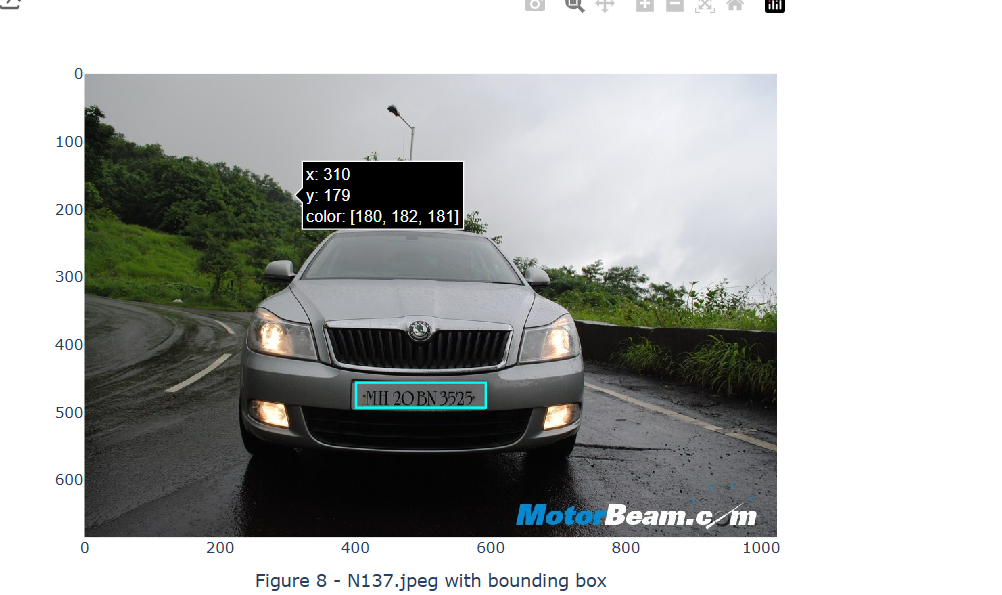
\includegraphics[width=10cm]{img/img1/Screenshot 2024-11-20 152513.png}

%3
\section{XỬ LÝ DỮ LIỆU}
\subsection{ĐỌC DỮ LIỆU}

Đây là một bước rất quan trọng, trong quá trình này, chúng ta sẽ lấy từng hình ảnh và chuyển đổi chúng thành một mảng bằng OpenCV và thay đổi kích thước hình ảnh thành 224 x 224, đây là kích thước tương thích tiêu chuẩn của mô hình học chuyển giao được đào tạo trước.\\
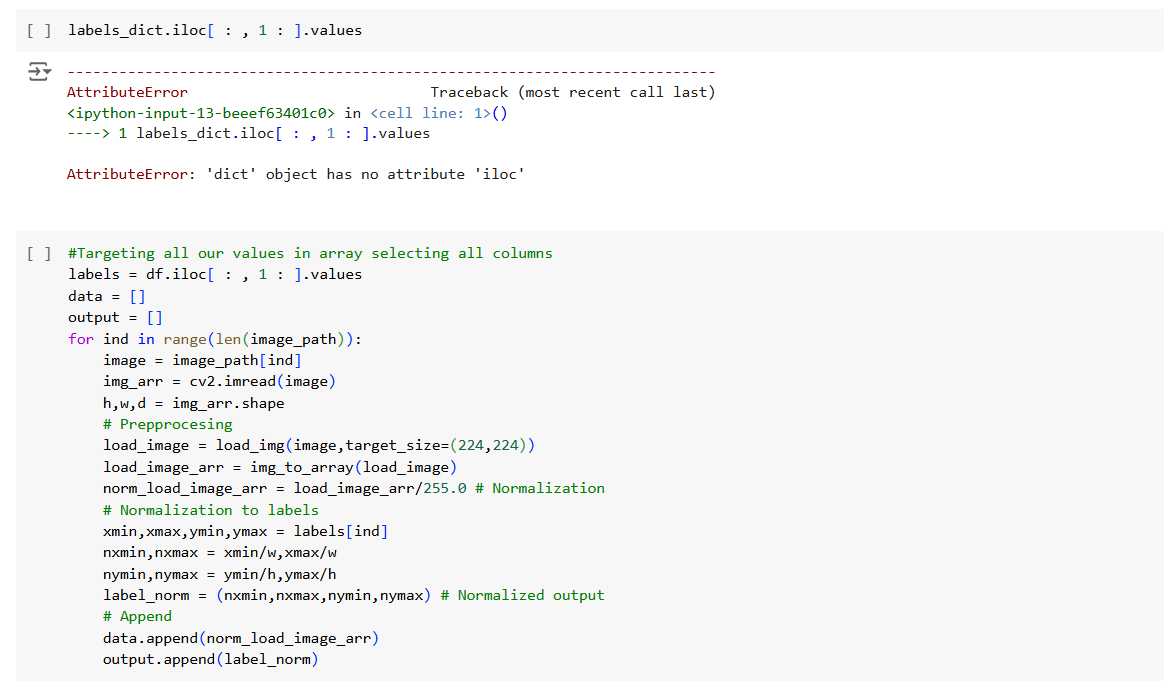
\includegraphics[width=10cm]{img/img1/3.1.png}\\
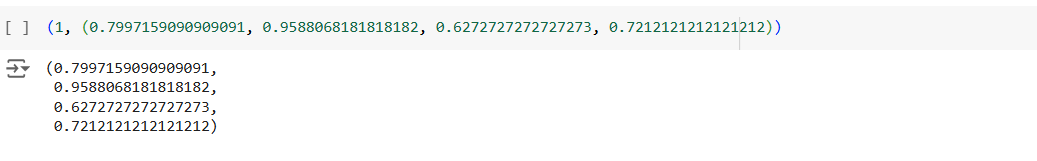
\includegraphics[width=10cm]{img/img1/3.1.1.png}\\

Sau đó, chúng ta sẽ chuẩn hóa hình ảnh chỉ bằng cách chia với số lượng lớn nhất vì chúng ta biết rằng số lượng lớn nhất cho một hình ảnh 8 bit là 28 -1 = 255. Đó là lý do tại sao chúng ta sẽ chia hình ảnh của mình thành 255.0. Cách chia một mảng với giá trị lớn nhất được gọi là Chuẩn hóa (Min-Max Scaler). Chúng ta cũng cần chuẩn hóa nhãn của mình nữa. Bởi vì đối với mô hình học sâu, phạm vi đầu ra phải nằm trong khoảng từ 0 đến 1. Để chuẩn hóa nhãn, chúng ta cần chia các điểm chéo với chiều rộng và chiều cao của hình ảnh. Và cuối cùng là các giá trị trong danh sách python.
\subsection{BỘ TẬP LUYỆN TÁCH VÀ KIỂM TRA }
In the next step, we will convert the list into an array using \textbf{Numpy}.\\
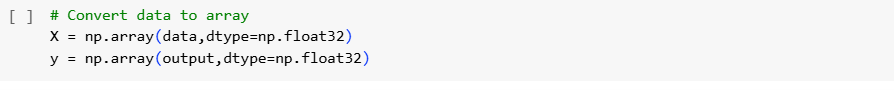
\includegraphics[width=10cm]{img/img1/3.2.png}\\
Bây giờ hãy chia dữ liệu thành tập huấn luyện và tập kiểm tra bằng \textbf{sklearn}.
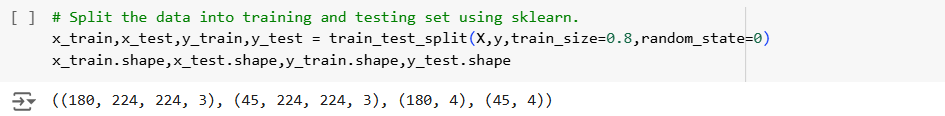
\includegraphics[width=10cm]{img/img1/3.2.2.png}\\


%4
\section {DEEP LEARNING FOR OBJECT DETECTION}
\subsection{XÂY DỰNG MÔ HÌNH INCEPTION-RESNET-V2}

 Inception-ResNet-V2 là một mạng nơ-ron tích chập được huấn luyện trên hơn một triệu hình ảnh từ cơ sở dữ liệu ImageNet. Mạng này có độ sâu 164 lớp và có khả năng phân loại hình ảnh vào 1000 danh mục đối tượng.

 Inception-ResNet-v2 được sử dụng cho nhiệm vụ phân loại. Inception-ResNet-v2 được xây dựng dựa trên sự kết hợp của cấu trúc Inception và kết nối dư thừa (Residual connection). Trong khối Inception-ResNet, các bộ lọc tích chập có kích thước khác nhau được kết hợp bởi các kết nối dư thừa. Việc sử dụng các kết nối dư thừa không chỉ tránh được vấn đề suy giảm hiệu suất do cấu trúc sâu gây ra mà còn giảm thời gian huấn luyện \\ 
 
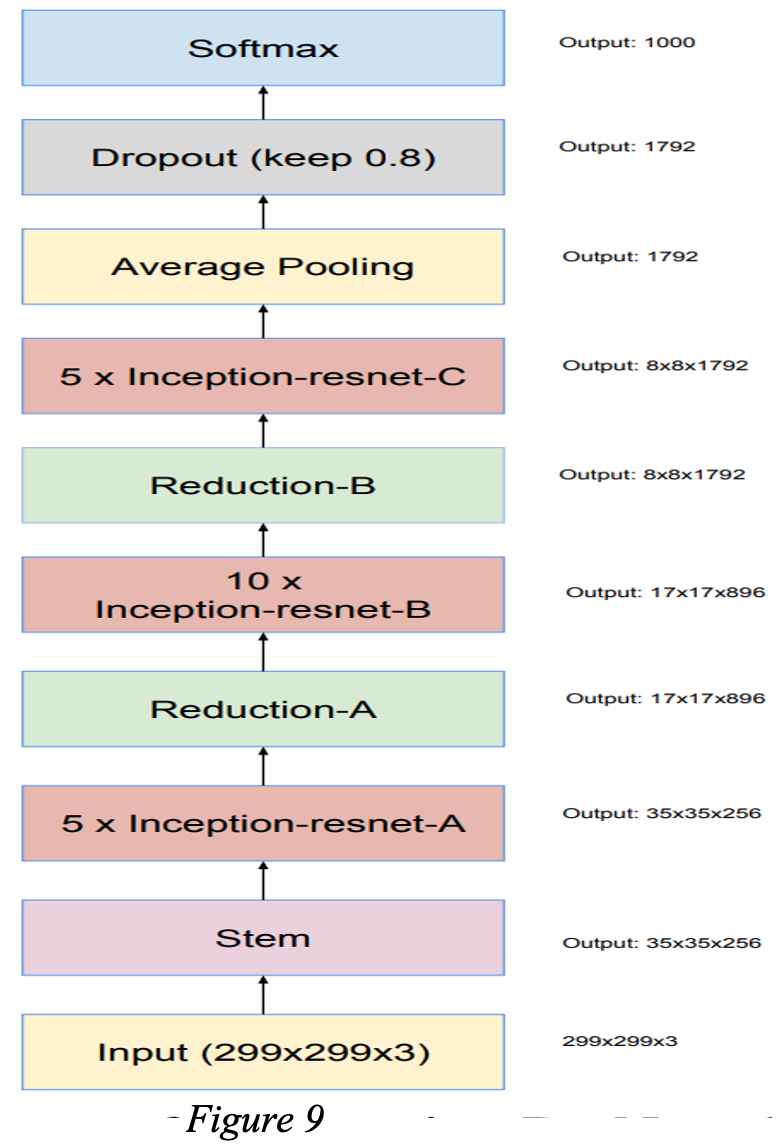
\includegraphics[width= 6cm]{img/img1/Notebook7.png} \\

Sử dụng mô hình Inception-ResNet-v2 với các trọng số đã được huấn luyện trước và huấn luyện mô hình này với dữ liệu. Nhập các thư viện cần thiết từ TensorFlow trước đó. \\

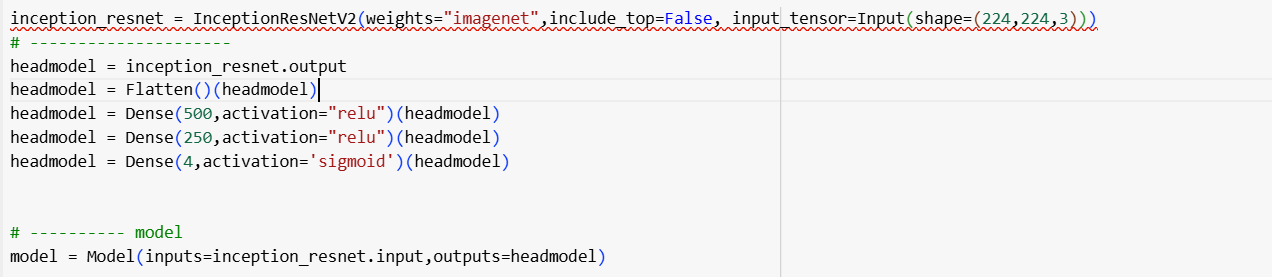
\includegraphics[width = 15cm]{img/img1/4.1.png} \\ 

Biên dịch mô hình và xem qua bản tóm tắt. Bản tóm tắt này bằng văn bản và bao gồm thông tin về: Các lớp và thứ tự của chúng trong mô hình. Hình dạng đầu ra của mỗi lớp. Số lượng tham số (trọng số) trong mỗi lớp.

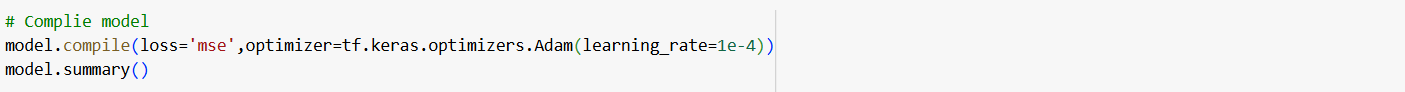
\includegraphics[width = 15cm]{img/img1/Screenshot 2024-11-20 161219.png}

\subsection{HUẤN LUYỆN VÀ LƯU TRỮ INCEPTION-RESNET-V2}
\hspace{2cm} \hl{$tfb = TensorBoard\textcolor{blue}{(}\textcolor{red}{'object\_detection'}\textcolor{blue}{)}$} \\

Đoạn mã này tạo ra một instance của callback TensorBoard và xác định thư mục để lưu các bản ghi. Những bản ghi này sau đó có thể được sử dụng để trực quan hóa quá trình huấn luyện với TensorBoard. \\

\hl{$history = 
model.fit\textcolor{blue}{(}x=x_train,y=y_train,batch_size=\textcolor{green}{10},epochs=\textcolor{green}{100},validation\_data=\textcolor{green}{(}x_test,y_test\textcolor{green}{)},callbacks=\textcolor{green}{[}tfb\textcolor{green}{]}\textcolor{blue}{)}$} \\

Đoạn mã này huấn luyện mô hình mạng nơ-ron với dữ liệu huấn luyện và xác thực đã cung cấp, đồng thời lưu lại các thông tin liên quan đến quá trình huấn luyện để có thể quan sát và phân tích sau này \\ 

\hl{$model.save\textcolor{blue}{(}\textcolor{red}{'./my\_model.keras'}\textcolor{blue}{)}$} \\


Đoạn mã này đảm bảo rằng có thể tải lại mô hình này sau để tiếp tục huấn luyện hoặc sử dụng để dự đoán mà không cần xây dựng lại từ đầu


\subsection{TENSORBOARD}

Cần chạy một lệnh đơn giản với đường dẫn đúng cho "object detection". Sau đó, sẽ thấy đầu ra với liên kết được lưu trữ, mở nó bằng Chrome. Sử dụng VSCode cho dự án này. Bây giờ, tôi sẽ cho bạn xem một ảnh chụp màn hình của kết quả mà chúng ta có. Chúng ta có thể thấy trên các scalar ở Hình 12, cách mà mô hình hoạt động. Bộ dữ liệu huấn luyện và xác thực không có hành vi overfitting và mất mát với mỗi epoch giảm dần.

Bạn chỉ cần gõ \hl{!tensorboard --logdir=\textquotedblleft./object\_detection\textquotedblright}  nó sẽ tạo ra một liên kết với văn bản, nhấp vào liên kết và chúng ta sẽ đi tiếp. \hl{Serving TensorBoard tại localhost; để mở rộng ra mạng, sử dụng proxy hoặc truyền --bind\_all TensorBoard 2.6.0 tại $\textcolor{blue}{\href{http://localhost:6006/}{http://localhost:6006/}}$ (Nhấn CTRL+C để thoát)} \\

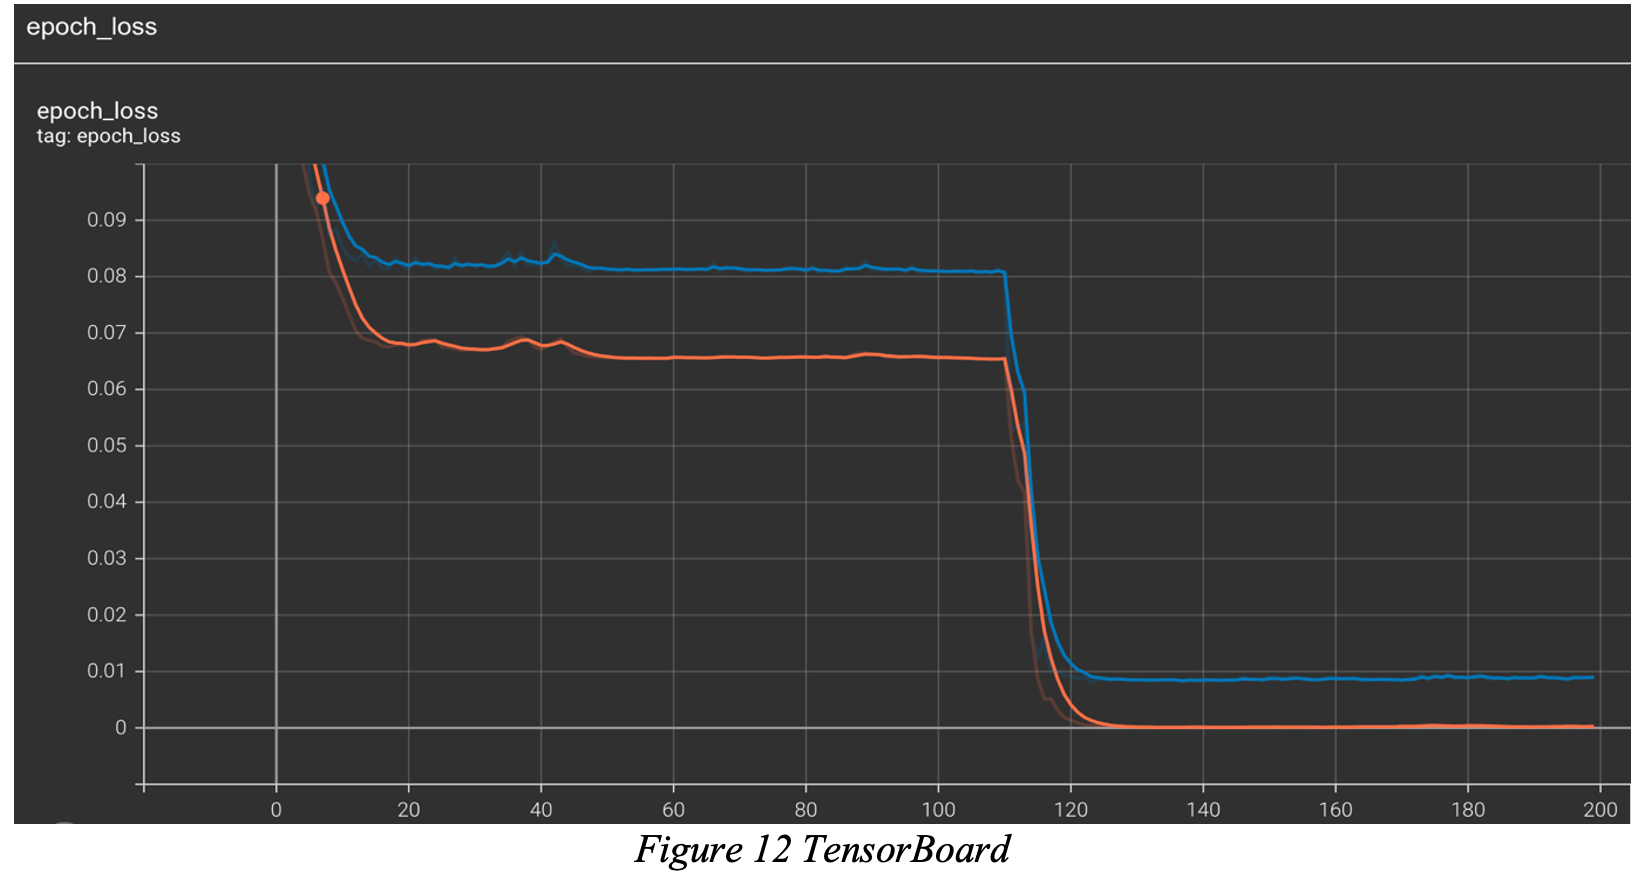
\includegraphics[width = 15cm]{img/img1/Notebook8.png}



%section 5
\section{MÔ HÌNH PHÁT HIỆN ĐỐI TƯỢNG THEO DÂY CHUYỀN}
\subsection{DỰ ĐOÁN}
Đây là bước cuối cùng trong việc phát hiện đối tượng. Trong bước này, chúng ta sẽ kết hợp tất cả lại và thực hiện dự đoán cho một hình ảnh cụ thể. Trước tiên, thử với một trong những bức ảnh thử nghiệm về ô tô của tôi.\\

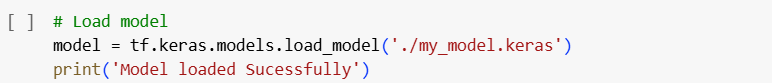
\includegraphics[width= 17cm]{img/img1/7.png}\\

Tiếp theo là tải ảnh TEST với đường dẫn đến nó.\\

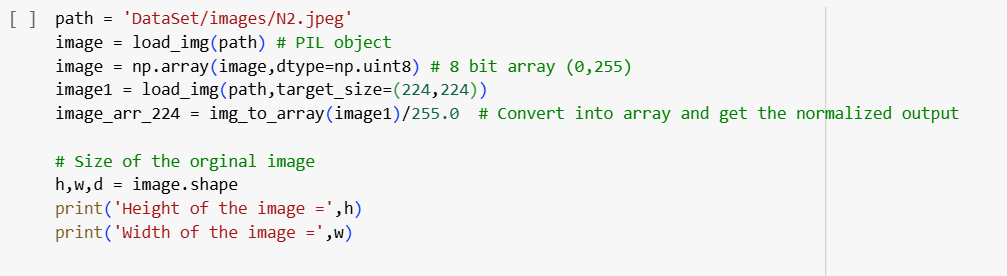
\includegraphics[width= 17cm]{img/img1/8.png}

Có thể xem hình  \\

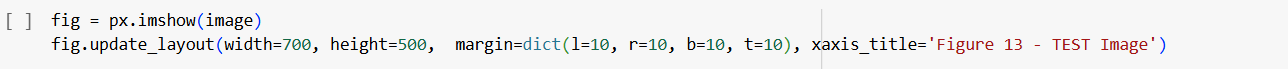
\includegraphics[width= 17cm]{img/img1/9.png}

Hãy nhìn vào shape của ảnh

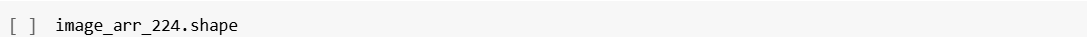
\includegraphics[width = 17cm]{img/img1/10.png}\\

output: (224, 224, 3)\\

Nhưng để truyền hình ảnh này qua mô hình, cần cung cấp dữ liệu trong chiều thứ tư động. Và những gì chỉ là một số hình ảnh. Vì vậy, ở đây chỉ truyền một hình ảnh duy nhất.\\

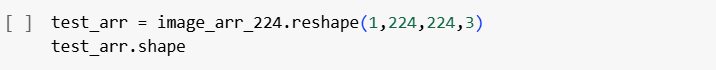
\includegraphics[width= 17cm]{img/img1/11.png}\\

output: (1, 224, 224, 3)\\
\subsection{KHỬ CHUẨN HÓA ĐẦU RA}
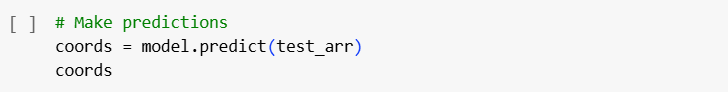
\includegraphics[width= 17cm]{img/img1/12.png}\\

output:\\
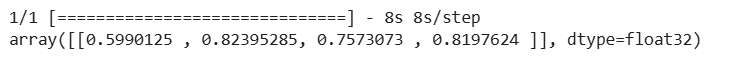
\includegraphics[width = 17cm]{img/img1/13.png}\\

Chúng ta đã nhận được đầu ra từ mô hình và đầu ra mà chúng ta có được là đầu ra đã được chuẩn hóa. Vì vậy, điều chúng ta cần làm là chuyển đổi lại thành các giá trị dạng gốc, điều mà chúng ta đã làm trong quá trình huấn luyện, trong quá trình huấn luyện, chúng ta có các giá trị dạng gốc và chuyển đổi nó thành giá trị chuẩn hóa. Vậy về cơ bản, chúng ta sẽ khử chuẩn hóa các giá trị này trở lại.

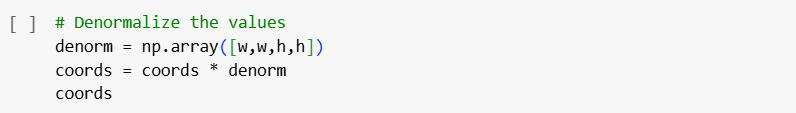
\includegraphics[width= 17cm]{img/img1/14.png}\\

output: array([[1864.1268816 , 2564.14128065, 1772.09906101, 1918.24403644]])



\subsection{HỘP GIỚI HẠN}
Bây giờ chúng ta sẽ vẽ hộp giới hạn lên trên hình ảnh. Tôi chỉ muốn cung cấp hai điểm chéo của hình ảnh. Hãy sử dụng các điểm này và vẽ hộp chữ nhật.\\

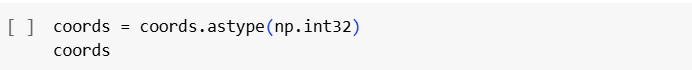
\includegraphics[width= 17cm]{img/img1/15.png}\\

output: array([[1864, 2564, 1772, 1918]], dtype=int32)\\

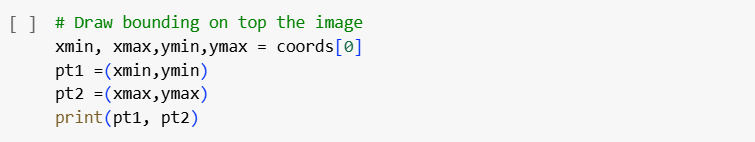
\includegraphics[width= 17cm]{img/img1/16.png}\\

output: (1864, 1772) (2564, 1918)

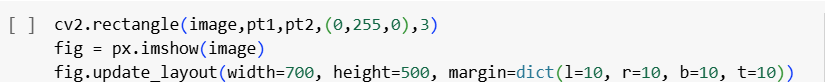
\includegraphics[width= 17cm]{img/img1/17.png}
\subsection{TẠO DÂY CHUYỀN}
Hãy đặt tất cả vào một chỗ và tạo hàm. Đầu ra sẽ trả về hình ảnh và tọa độ của hộp giới hạn.

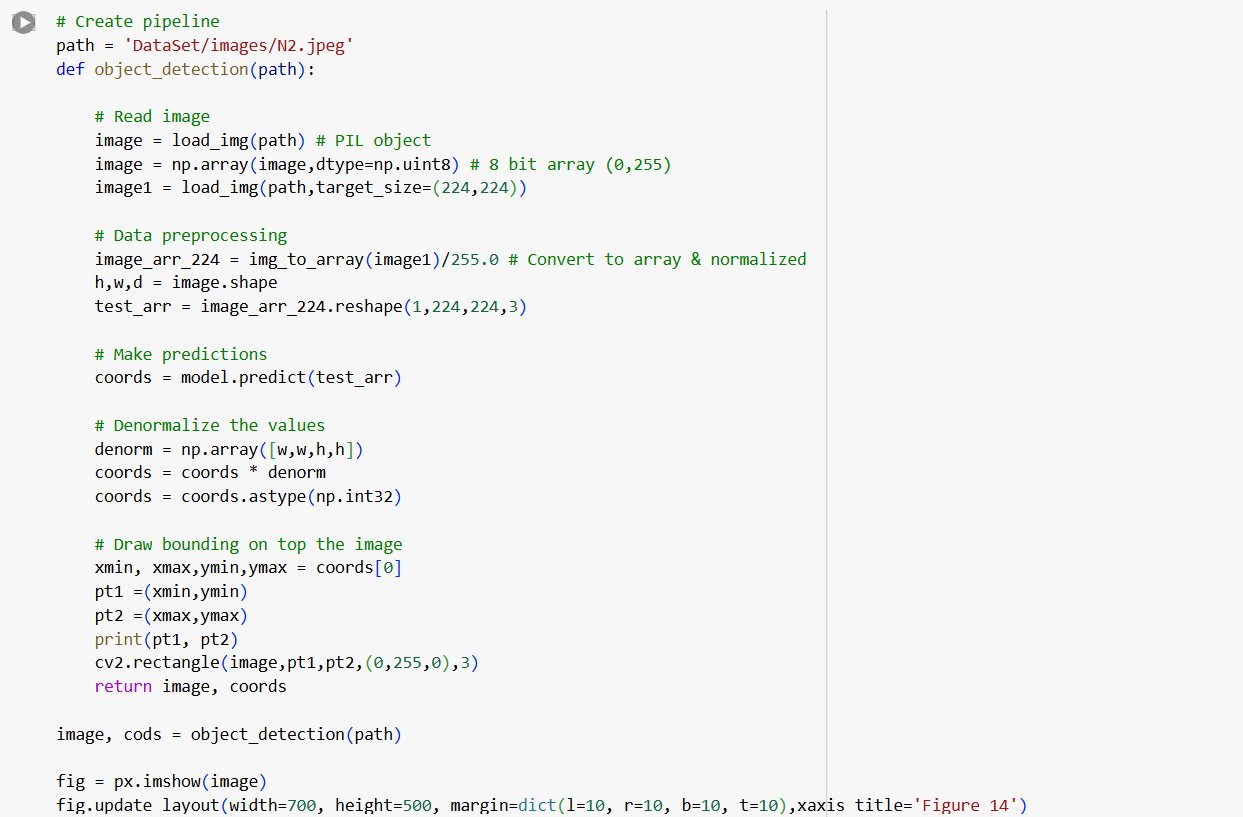
\includegraphics[width= 17cm]{img/img1/18.png}

%phần 6
\section{NHẬN DẠNG KÝ TỰ QUANG HỌC - OCR}
\subsection{TESSERACT OCR}
Phần mềm nhận dạng ký tự quang học (OCR) được sử dụng để trích xuất văn bản từ hình ảnh. Tesseract OCR có API python và nó là nguồn mở. Đầu tiên chúng ta sẽ tiến hành cài đặt nó. Nó khá đơn giản và phụ thuộc vào hệ điều hành của bạn. Bạn có thể tìm thấy hướng dẫn sử dụng và các tập tin để tải xuống để cài đặt
\href{https://guides.library.illinois.edu/c.php?g=347520&p=4121425.}{\textcolor{blue}{tại đây}}
\subsection{HẠN CHẾ CỦA PYTESSERACT}
Tesseract hoạt động tốt nhất khi có sự phân chia rõ ràng giữa văn bản nền trước và nền. Trong thực tế, việc đảm bảo các kiểu thiết lập này có thể cực kỳ khó khăn. Có nhiều lý do khiến bạn không thể nhận được đầu ra chất lượng tốt từ Tesseract, chẳng hạn như hình ảnh có nhiễu trên nền. Chất lượng hình ảnh càng tốt (kích thước, độ tương phản, độ sáng) thì kết quả nhận dạng càng tốt. Nó đòi hỏi một chút tiền xử lý để cải thiện kết quả OCR, hình ảnh cần được chia tỷ lệ phù hợp, có độ tương phản hình ảnh càng cao càng tốt và văn bản phải được căn chỉnh theo chiều ngang. Tesseract OCR khá mạnh nhưng có những hạn chế sau.

Giới hạn Tesseract được tóm tắt trong danh sách.
\begin{itemize}

\item OCR không chính xác như một số giải pháp thương mại hiện có của chúng tôi.

\item Không hoạt động tốt với những hình ảnh bị ảnh hưởng bởi các thành phần giả bao gồm che khuất một phần, phối cảnh bị bóp méo và nền phức tạp.

\item Nó không có khả năng nhận dạng chữ viết tay.
\item Nó có thể tìm thấy những từ vô nghĩa và báo cáo đây là đầu ra OCR.
\item Nếu tài liệu chứa các ngôn ngữ nằm ngoài ngôn ngữ được đưa ra trong đối số -l LANG thì kết quả có thể kém.

\item Không phải lúc nào cũng tốt trong việc phân tích thứ tự đọc tự nhiên của tài liệu. Ví dụ: nó có thể không nhận ra rằng tài liệu có chứa hai cột và có thể cố gắng nối văn bản trên các cột.

\item Quét chất lượng kém có thể tạo ra OCR chất lượng kém.
\item Nó không tiết lộ thông tin về văn bản thuộc họ phông chữ nào.

\end{itemize}
\subsection{TRÍCH DẪN VĂN BẢN BIỂU SỐ TỪ HÌNH ẢNH}
Đầu tiên, chúng ta sẽ tải hình ảnh của mình và chuyển đổi thành mảng. Cắt hộp giới hạn của chúng tôi với tọa độ của nó. Chúng tôi sẽ xác định vùng quan tâm (ROI) và xem hình ảnh đã cắt của chúng tôi Hình 15.
\setlength{\parindent}{1cm}
\begin{verbatim}
    img = np.array(load_img(path))
xmin ,xmax,ymin,ymax = cods[0]
roi = img[ymin:ymax,xmin:xmax]
fig = px.imshow(roi)
fig.update_layout(width=350, height=250, margin=dict(l=10, r=10,
b=10,t=10),xaxis_title='Figure 15 Cropped image')
\end{verbatim}
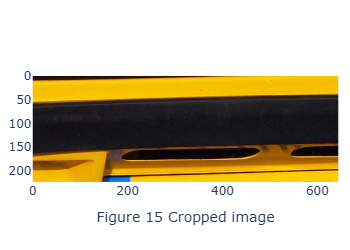
\includegraphics[width= 7cm]{img/img/newplot.png}\\
Với việc sử dụng Tesseract, chúng ta sẽ trích xuất văn bản từ hình ảnh

\begin{verbatim}
    # extract text from image
text = pt.image_to_string(roi)
print(text)
\end{verbatim}

42-UK-32
\\

Rõ ràng là chúng tôi không nhận được văn bản phù hợp, nhưng ít nhất bạn có thể lấy được 90\% thông tin. Nó chỉ là một ví dụ và một lần nữa sẽ cần phải nói rằng càng nhiều dữ liệu thì càng có nhiều dự đoán tốt hơn. Chúng ta sẽ đến thời điểm đó trong tương lai. Điều tôi nhận ra ở đây: Trước hết, chúng tôi không có nhiều dữ liệu, để giải quyết vấn đề này và tôi đã thêm vào chủ đề này nhiều bộ dữ liệu gần như giống với các bộ dữ liệu từ các kaggler khác được đăng gần đây. Thứ hai, tôi không thấy mô hình này hoạt động tốt, thành thật mà nói với bạn, nhưng toàn bộ quá trình đã được thực hiện đã mang lại cơ hội để hiểu rõ khái niệm, chúng tôi sẽ xây dựng một mô hình khác với sự trợ giúp của YOLO và nơi chúng tôi có thể xem nó hoạt động như thế nào kết quả của chúng tôi. Phần thứ hai của Tesseract, tôi đã giải thích một số giới hạn của nó, nhưng việc xử lý trước hình ảnh có thể là một chủ đề khác và thậm chí có thể yêu cầu xây dựng AI trên đó. Vì vậy, bây giờ tôi muốn bạn chỉ cho bạn cách xây dựng trang web đơn giản và bước tiếp theo sau đó chúng ta sẽ bắt đầu với mô hình mới.

%7
\section{ỨNG DỤNG WEB BIỂU SỐ}
Phần này tôi sẽ giải thích ngắn gọn tất cả về cách cài đặt và tích hợp nó vào web. Tôi hiểu rằng một số bước có thể tự giải thích nhưng tôi thực hiện nó theo cách thủ công và nếu nó giúp ích cho một người trong danh sách thì điều đó có ý nghĩa gì đó đối với tôi. Trong trường hợp khác, bạn có thể bỏ qua vài bước và uống vài ly cà phê.
\subsection{CÔNG CỤ BẮT BUỘC}
Để chạy dự án của chúng tôi và chúng tôi cần cài đặt \href{https://code.visualstudio.com/download.}{VSCode} 
và một số tiện ích mở rộng quan trọng mà bạn có thể tìm thấy trong danh sách bên dưới. Tiện ích mở rộng sẽ giúp chúng tôi trong tương lai.
\begin{itemize}
    \item \href{https://marketplace.visualstudio.com/items?itemName=Atishay-Jain.All-Autocomplete.}{All autocomplete}\\
    \item \href{https://marketplace.visualstudio.com/items?itemName=donjayamanne.python-extension-pack.}{Python extension pack}\\
    \item \href{https://marketplace.visualstudio.com/items?itemName=redhat.vscode-yaml.}{Yaml}\\
    \item \href{https://marketplace.visualstudio.com/items?itemName=thekalinga.bootstrap4-vscode.}{Bootstrap 4, font awesome 4, font awesome 5 free & pro snippets}\\
    \item \href{https://marketplace.visualstudio.com/items?itemName=batisteo.vscode-django.}{Django}\\
    \item \href{https://marketplace.visualstudio.com/items?itemName=sidthesloth.html5-boilerplate.}{Html boilerplate}\\
    \item \href{https://marketplace.visualstudio.com/items?itemName=abusaidm.html-snippets.}{Html snippets}
    \item \href{https://marketplace.visualstudio.com/items?itemName=cstrap.flask-snippets.}{Flask-snippets}\\

\end{itemize}
\subsection{ Ứng dụng Flask.}
Đầu tiên, hãy đảm bảo cài đặt Flask.
\textcolor{white}{\hl{!pip install flask}} Và đóng gói tập tin mới App.py.
\begin{verbatim}
flask import Flask

# Webserver gateway interface
app = Flask (__name__)

@app.route('/')
def index():
    return "Hello World"

if __name__ =="__main__":
    app.run()>}}
\end{verbatim}
Chạy như trên thiết bị đầu cuối (đảm bảo bạn đang ở trong cùng thư mục nơi bạn dự án.) Bạn sẽ thấy kết quả như thế này \textcolor{white}{\hl{Running on http://127.0.0.1:5000 (Press CTRL+C to quit)}}
Mở URL trên Chrome để kiểm tra Hình 16\\
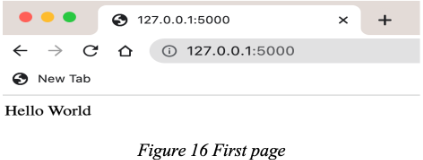
\includegraphics[width= 8cm]{img/img1/Screenshot 2024-11-20 193708.png}
\\
Tiếp theo tạo các mẫu thư mục trong dự án của chúng tôi trong các mẫu thư mục tạo tệp mới dưới dạng bố cục.html. Vì chúng tôi đã cài đặt các tiện ích mở rộng, chỉ cần gõ html và chọn bản soạn sẵn, bạn sẽ thấy nội dung như trên Hình 17 và !DOCTYPE html


\\
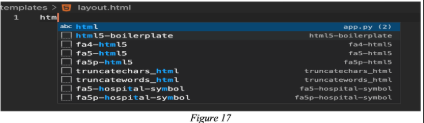
\includegraphics[width= 8cm]{img/img1/Screenshot 2024-11-20 194057.png}
\begin{verbatim}
<!DOCTYPE html>

<html>
    <head>
        <meta charset="utf-8">
        <meta http-equiv="X-UA-Compatible" content="IE=edge">
        <title></title>
        <meta name="description" content="">
        <meta name="viewport" content="width=device-width, initial-scale=1">
        <link rel="stylesheet" href="">
    </head>
    <body>
        <!--[if lt IE 7]>
            <p class="browsehappy">You are using an <strong>outdated</strong> browser. Please <a href="#">upgrade your browser</a> to improve your experience.</p>
        <![endif]-->

        <script src="" async defer></script>
    </body>
</html>
\end{verbatim}
Và bây giờ chúng ta có thể bắt đầu xây dựng trang của mình. Chúng tôi có thể thay đổi Tiêu đề và thêm loại nội dung, v.v. Chúng tôi sẽ cần sửa đổi app.py, bố cục (và Bootstrap thành bố cục mà bạn có thể tìm thấy \href{https://getbootstrap.com/docs/5.2/getting-started/introduction/.}{link}
ở đây chúng tôi rất thú vị) và thêm chân trang. Ở giai đoạn này nó sẽ trông như dưới đây.
\textcolor{white}{\hl{app.py}}
\begin{verbatim}
from flask import Flask, render_template

# Webserver gateway interface
app = Flask(__name__)

@app.route('/')
def index():
    return render_template('layout.html')

if __name__ == "__main__":
    app.run(debug=True)
\end{verbatim}

\textcolor{white}{\hl{layout.html}}

\begin{verbatim}
<!DOCTYPE html>

<html>
  <head>
    <meta charset="utf-8" />
    <meta http-equiv="X-UA-Compatible" content="IE=edge" />
    <title>AUTOMATIC NUMBER-PLATE RECOGNITION</title>
    <link
      href="https://cdn.jsdelivr.net/npm/bootstrap@5.2.0-beta1/dist/css/bootstrap.min.css"
      rel="stylesheet"
      integrity="sha384-0evHe/X+R7YkIZDRvuzKMRqM+OrBnVFBL6DOitfPri4tjfHxaWutUpFmBp4vmVor"
      crossorigin="anonymous"
    />
    <script
      src="https://cdn.jsdelivr.net/npm/bootstrap@5.2.0-beta1/dist/js/bootstrap.bundle.min.js"
      integrity="sha384-pprn3073KE6tl6bjs2QrFaJGz5/SUsLqktiwsUTF55Jfv3qYSDhgCecCxMW52nD2"
      crossorigin="anonymous"
    ></script>
    <meta name="description" content="" />
    <meta name="viewport" content="width=device-width, initial-scale=1" />
    <link rel="stylesheet" href="" />
  </head>
  <body>
    <!-- Navigation bar -->
    <nav class="navbar navbar-light" style="background-color: #c1dce0">
      <div class="container">
        <a class="navbar-brand" href="/">
          <h1 class="display-6">NUMBER PLATE OCR</h1>
        </a>
      </div>
    </nav>
    <!-- Footer -->
    <footer>
      <hr />
      <a href="http://aslanahmedov.com"> CONTACT ME</a>
    </footer>
    <script src="" async defer></script>
  </body>
</html>
\end{verbatim}
\subsection{Kế thừa MẪU}
\textcolor{white}{\hl{Chúng tôi sẽ tạo tệp mới dưới dạng html và đặt tên là index.html và chúng tôi dự định viết tất cả chức năng ra ngoài index.html. Trước tiên, hãy truy cập vào bố cục.html bên dưới khối nội dung của chúng tôi - xem bên dưới.}}
\begin{verbatim}
</nav>
    

    
\end{verbatim}

Trong index.html chúng ta cần mở rộng bố cục.html và chặn phần thân của nó như bên dưới.
\begin{verbatim}



\end{verbatim}
\textcolor{white}{\hl{In app.py change layout.html to index.html and save it. CTRL+S always-everywhere! We will add some forms as well to index.html see below.}}
\begin{verbatim}


<div class="container">
  <br /><br /><br />
  <form action="#" method="POST" enctype="multipart/form-data">
    <div class="input-group">
      <input type="file" class="form-control" name="image_name" required />
      <input type="submit" value="UPLOAD" class="btn btn-outline-secondary" />
    </div>
  </form>
</div>  
\end{verbatim}
\subsection{Phương thức HTTP để tải lên tệp trong Flask.}
\begin{verbatim}
from flask import Flask, render_template, request
import os
# Webserver gateway interface
app = Flask(__name__)

BASE_PATH = os.getcwd()
UPLOAD_PATH = os.path.join(BASE_PATH, 'static/upload/')

@app.route('/', methods=['POST'])
def index():
    if request.method == 'POST':
        upload_file = request.files['image_name']
        filename = upload_file.filename
        path_save = os.path.join(UPLOAD_PATH,filename)
        upload_file.save(path_save)


        return render_template('index.html')

    return render_template('index.html')

if __name__ == "__main__":
    app.run(debug=True)
\end{verbatim}
\subsection{Tích hợp NPD và OCR vào ứng dụng Flask.}
Bây giờ chúng ta sẽ sử dụng hình ảnh đã tải lên và thực hiện dự đoán bằng mô hình học sâu. Đầu tiên, chúng ta sẽ tạo thêm một tệp và đặt tên là deeplearning.py, trong tệp này chúng ta sẽ đơn giản thêm toàn bộ pipeline của mình, bao gồm tất cả các thư viện và hàm cần thiết với đường dẫn chính xác đến mô hình. Đồng thời, tạo thêm hai thư mục là roi và predict trong thư mục static. Cuối cùng, mã của bạn sẽ trông giống như sau 
\href{https://github.com/Asikpalysik/Automatic-License-Plate Detection/blob/main/WebbApp/deeplearning.py}{đây}
Trên Flask cũng vậy, 'thêm văn bản' - bạn có thể tìm thấy nó \href{https://github.com/Asikpalysik/Automatic-License-Plate Detection/blob/main/WebbApp/app.py}{ở đây}
Vậy là chúng ta gần hoàn thành. Bây giờ khi chúng ta tải lên hình ảnh của chiếc xe có số biển, mô hình của chúng ta sẽ dự đoán bounding box, cắt nó ngay lập tức, lưu các kết quả vào thư mục roi và thư mục predict. Để hiển thị trên web, chúng ta sẽ chỉnh sửa tệp index.html và thêm tính năng lưu văn bản. Bạn có thể tìm thấy mã đã sẵn sàng.\href{https://github.com/Asikpalysik/Automatic-License-Plate-Detection/blob/main/WebbApp/templates/index.html}{ở đây}
Và trong Hình 19, bạn có thể thấy kết quả. Tất cả các tệp và thư mục cho Web, vui lòng kiểm tra thoải mái.\href{https://github.com/Asikpalysik/Automatic-License-Plate-Detection/tree/main/WebbApp}{ở đây}
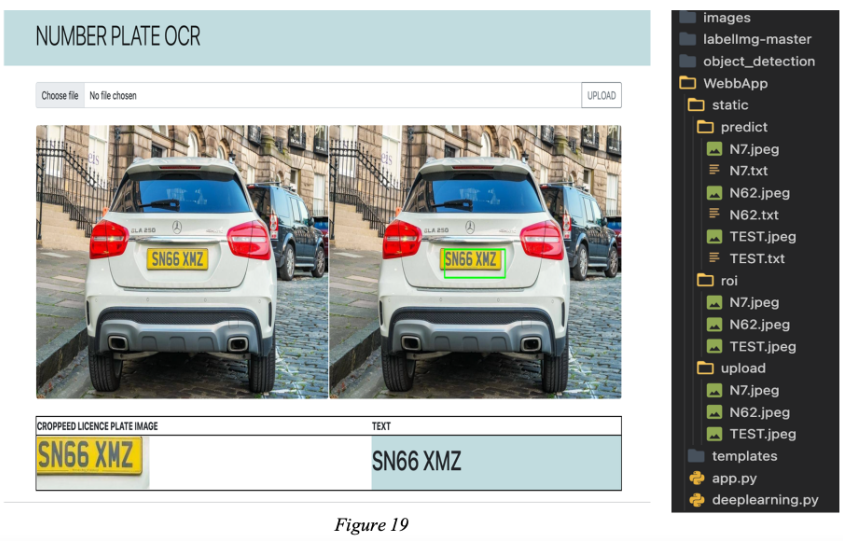
\includegraphics[width= 10cm]{img/img/Screenshot 2024-11-20 201114.png}


%8
\section{Nhận diện biển số xe thời gian thực bằng YOLO}
\subsection{Giải thích về dữ liệu cần thiết}
YOLO, viết tắt của "You Only Look Once", là một trong những thuật toán phát hiện đối tượng dựa trên học sâu được sử dụng rộng rãi nhất hiện nay. YOLO chia một hình ảnh thành một hệ thống lưới, và mỗi ô trong lưới sẽ phát hiện các đối tượng bên trong nó. Thuật toán này có thể được sử dụng để phát hiện đối tượng trong thời gian thực dựa trên các luồng dữ liệu, đồng thời yêu cầu rất ít tài nguyên tính toán.
Kiến trúc mạng của YOLOv5 bao gồm ba phần chính:
\begin{itemize}
    \item Kiến trúc mạng của YOLOv5 bao gồm ba phần chính:
    \item Neck: PANet (được sử dụng để hợp nhất các đặc trưng).
    \item Head: Yolo Layer (xuất ra kết quả phát hiện).
\end{itemize}
Dữ liệu đầu vào được truyền trước tiên qua CSPDarknet để trích xuất đặc trưng, sau đó được đưa vào PANet để hợp nhất các đặc trưng. Cuối cùng, Yolo Layer sẽ xuất ra kết quả phát hiện, bao gồm loại đối tượng, điểm số, vị trí và kích thước.\\
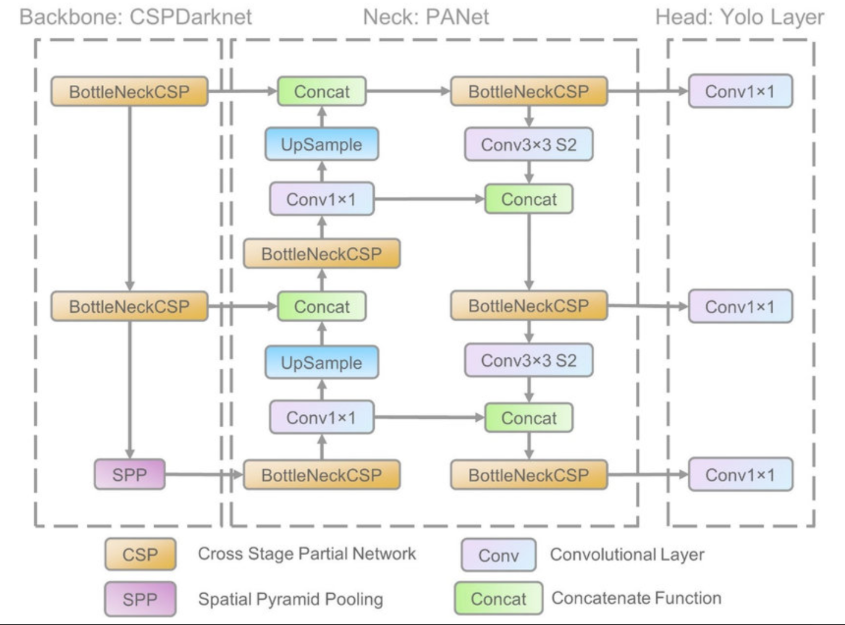
\includegraphics[width= 10cm]{img/img/Screenshot 2024-11-21 192454.png}
Quy trình trước đây của chúng ta rất tốt, nhưng mô hình hiện tại gặp một số vấn đề. Vấn đề lớn nhất là mô hình có độ chính xác rất thấp trong việc phát hiện biển số xe, đồng thời tốc độ xử lý cũng rất chậm. Để khắc phục những hạn chế trên, đặc biệt là vấn đề độ chính xác, chúng ta sẽ sử dụng mô hình giảm thiểu mạnh mẽ nhất cho đến nay, đó là YOLO.

Bây giờ, hãy cùng xem cách chúng ta có thể sử dụng quy trình chuẩn bị dữ liệu hiện tại cho mô hình YOLO. Công việc gán nhãn và tiền xử lý dữ liệu mà chúng ta đã thực hiện trước đây vẫn có thể áp dụng cho mô hình YOLO. Tuy nhiên, có một sự khác biệt lớn mà chúng ta cần thực hiện trong YOLO, đó là định dạng nhãn.

Trước đây, như bạn đã thấy, chúng ta sử dụng các giá trị xmin, xmax, ymin, ymax làm đầu ra thực tế. Nhưng đối với YOLO, nhãn đầu ra sẽ là tọa độ X-Y trung tâm của hộp giới hạn và chiều rộng (W), chiều cao (H) của hộp giới hạn. Đặc biệt, tọa độ X-Y sẽ được tính từ tâm của hộp giới hạn.

Ví dụ, hãy xem Hình 20. Đối với hình ảnh này, nhãn gán cho YOLO nên là tọa độ trung tâm X và Y, và tọa độ này cần được chuẩn hóa theo chiều rộng và chiều cao của hình ảnh. Tương tự, W (chiều rộng) và H (chiều cao) của hộp giới hạn cũng cần được chuẩn hóa theo chiều rộng và chiều cao của hình ảnh.\\

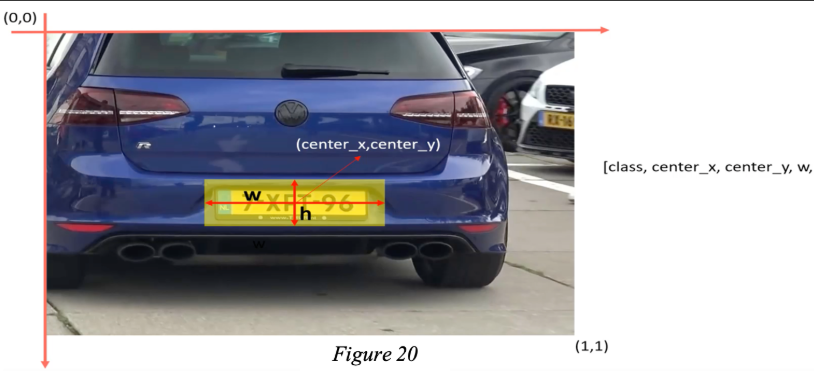
\includegraphics[width = 10cm]{img/img/Screenshot 2024-11-21 193015.png}
$
Vì vậy, trong quá trình gán nhãn, định dạng dữ liệu mà chúng ta cần chuẩn bị bây giờ sẽ bao gồm vị trí trung tâm của X, vị trí trung tâm của Y (liên quan đến hộp giới hạn), cùng với chiều rộng (width) và chiều cao (height) của hộp giới hạn. Định dạng sẽ như sau:[class, center_x, center_y, w, h] Đây là một trong những thay đổi mà chúng ta cần thực hiện.
\\
Ngoài ra, cấu trúc thư mục cần được chuẩn bị, đặc biệt dành cho YOLO, sẽ trông giống như minh họa trong Hình 21.\\
$
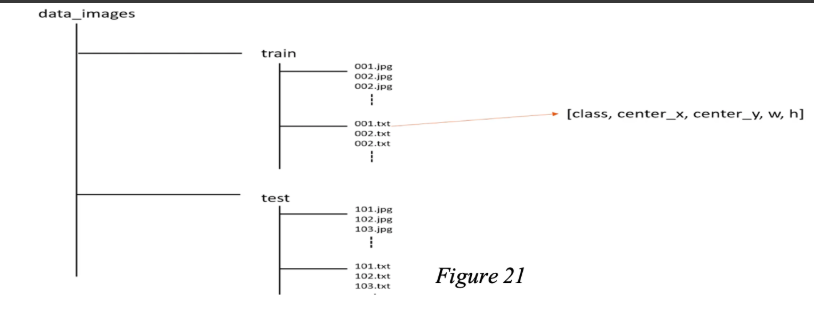
\includegraphics[width = 10cm]{img/img/Screenshot 2024-11-21 193724.png}

Hãy xem xét dữ liệu hình ảnh. Bên trong thư mục chứa dữ liệu hình ảnh, chúng ta cần tổ chức theo cách có thư mục train và test. Trong thư mục train, chúng ta sẽ lưu tất cả các hình ảnh liên quan đến việc huấn luyện và các nhãn tương ứng phải được lưu ở định dạng .txt. Thêm vào đó, thông tin nhãn phải có cùng tên với tệp hình ảnh. Tương tự như dữ liệu huấn luyện, chúng ta cũng sẽ chuẩn bị dữ liệu kiểm tra (test data).

Tôi sẽ viết một hàm để trích xuất thông tin về chiều rộng, chiều cao của hình ảnh và tên tệp từ các tệp định dạng XML. Việc tạo một hàm để phân tích cú pháp (parsing) và trả về các thông tin như tên tệp, chiều rộng, chiều cao, sau đó áp dụng chúng vào DataFrame sẽ được thực hiện như ví dụ bên dưới.
\begin{verbatim}
# parsing
def parsing(path):
    parser = xet.parse(path).getroot()
    name = parser.find('filename').text
    filename = f'/content/Automatic-License-Plate-Detection/images/{name}'

    # width and height
    parser_size = parser.find('size')
    width = int(parser_size.find('width').text)
    height = int(parser_size.find('height').text)

    return filename, width, height
df[['filename','width','height']] = df['filepath'].apply(parsing).apply(pd.Series)
df.head()
\end{verbatim}
$
Bước tiếp theo là tính toán center_x, center_y, width và height, được chuẩn hóa theo chiều rộng và chiều cao của hình ảnh. Đồng thời, chuẩn hóa chiều rộng và chiều cao của hộp giới hạn (bounding box).
$
\begin{verbatim}
# center_x, center_y, width , height
df['center_x'] = (df['xmax'] + df['xmin'])/(2*df['width'])
df['center_y'] = (df['ymax'] + df['ymin'])/(2*df['height'])

df['bb_width'] = (df['xmax'] - df['xmin'])/df['width']
df['bb_height'] = (df['ymax'] - df['ymin'])/df['height']
df.head()
\end{verbatim}
\subsection{Chuẩn bị Dữ liệu}

Một trong những thử thách lớn khi huấn luyện YOLO là phần cứng. YOLO yêu cầu một vi xử lý xử lý nhanh để huấn luyện. Việc huấn luyện YOLO trên các CPU thông thường là cực kỳ khó khăn. Đầu tiên, chúng ta phải sao chép YOLOv5 vào không gian làm việc của mình. Bạn có thể tìm thấy nó \href{https://github.com/ultralytics/yolov5}{ở đây}
Và cài đặt tất cả các yêu cầu. Hãy chắc chắn rằng bạn đang ở trong thư mục đúng như dưới đây, hãy làm theo nhé.\\
\textcolor{white}{\hl{!git clone https://github.com/ultralytics/yolov5}}
\\
$
Chúng ta cần tạo thêm một thư mục nữa và bên trong đó tạo hai thư mục con, đặt tên là data_images, train và test. Chúng ta sẽ phân chia dữ liệu thành hai phần: huấn luyện (train) và kiểm tra (test).$
\begin{verbatim}
mkdir yolov5/data_images/

mkdir yolov5/data_images/test/

mkdir yolov5/data_images/train/
    

### split the data into train and test
df_train = df.iloc[:200]
df_test = df.iloc[200:]
\end{verbatim}

Chúng ta sẽ sao chép từng hình ảnh vào các thư mục train và test và tạo ra các tệp .txt chứa thông tin nhãn
\begin{verbatim}
import shutil
import os
train_folder = 'yolov5/data_images/train'

values = df_train[['filename','center_x','center_y','bb_width','bb_height']].values
for fname, x,y, w, h in values:
    image_name = os.path.split(fname)[-1]
    txt_name = os.path.splitext(image_name)[0]

    dst_image_path = os.path.join(train_folder,image_name)
    dst_label_file = os.path.join(train_folder,txt_name+'.txt')
    print(fname)
    print(dst_image_path)
    if os.path.exists(fname):
      shutil.copy(fname, dst_image_path)
    else:
      print(f"The file {fname} does not exist.")
\end{verbatim}
\begin{verbatim}
import shutil
train_folder = 'yolov5/data_images/train'

values = df_train[['filename','center_x','center_y','bb_width','bb_height']].values
for fname, x,y, w, h in values:
    image_name = os.path.split(fname)[-1]
    txt_name = os.path.splitext(image_name)[0]

    dst_image_path = os.path.join(train_folder,image_name)
    dst_label_file = os.path.join(train_folder,txt_name+'.txt')
    print(fname)
    print(dst_image_path)
    # copy each image into the folder
    shutil.copy(fname,dst_image_path)

    # generate .txt which has label info
    label_txt = f'0 {x} {y} {w} {h}'
    with open(dst_label_file,mode='w') as f:
        f.write(label_txt)

        f.close()

test_folder = 'yolov5/data_images/test'

values = df_test[['filename','center_x','center_y','bb_width','bb_height']].values
for fname, x,y, w, h in values:
    image_name = os.path.split(fname)[-1]
    txt_name = os.path.splitext(image_name)[0]

    dst_image_path = os.path.join(test_folder,image_name)
    dst_label_file = os.path.join(test_folder,txt_name+'.txt')

    # copy each image into tahe folder
    copy(fname,dst_image_path)

    # generate .txt which has label info
    label_txt = f'0 {x} {y} {w} {h}'
    with open(dst_label_file,mode='w') as f:
        f.write(label_txt)

        f.close()
\end{verbatim}

Ngoài ra, tôi sẽ tạo tệp data.yaml với đường dẫn đến thư mục train và validation, cùng với số lượng lớp là 1, và đặt tên lớp trong danh sách là license plate. Bạn cần lưu tệp này trong bộ dữ liệu của mình vì chúng ta sẽ cần cung cấp đường dẫn đến tệp này sau.
\begin{verbatim}
train: data_images/train
val: data_images/test
nc: 1
names: [
    'license_plate'
]
\end{verbatim}
\subsection{TRAINING YOLO}
Bước tiếp theo là huấn luyện mô hình. Việc này có thể mất thời gian, vì vậy hãy chuẩn bị sẵn sàng. Bạn có thể sử dụng Kaggle hoặc Google Colab để thực hiện. Chúng ta đã chuẩn bị tệp data.yaml, giờ hãy cung cấp đường dẫn đến tệp đó và huấn luyện mô hình.
\begin{verbatim}
!python ./yolov5/train.py --data ./data.yaml --cfg ./yolov5/models/yolov5s.yaml --batch-size 8 --name Model --epochs 5
\end{verbatim}

Khi mô hình được huấn luyện xong, chúng ta cần lưu mô hình để sử dụng trong OCR ở định dạng onnx như sau:
\begin{verbatim}
!python ./yolov5/export.py --weight ./yolov5/runs/train/Model/weights/best.pt --include torchscript onnx
\end{verbatim}
$
Được rồi, chúng ta đã thành công trong việc lưu mô hình sau khi giải nén nó. Chúng ta có thể nhận thấy rằng có một thư mục mô hình. Trong đó, chúng ta có thể tìm thấy các hình ảnh dự đoán và mô hình của chúng ta có thể phát hiện biển số xe rất chính xác. Có thể sẽ có một vài kết quả sai, nhưng nhìn chung, mô hình của chúng ta phát hiện biển số xe rất chính xác. PR curve cuối cùng là rất quan trọng đối với tôi vì nó sẽ cho biết tỷ lệ phát hiện. Chúng ta có thể thấy rằng độ chính xác và độ thu hồi của mô hình cho thấy chúng ta có thể phát hiện biển số với Precision là 0.92 và Mean Average Precision (mAP) là 0.5. Bạn có thể xem ví dụ về một trong các val_batch dưới đây.\\
$
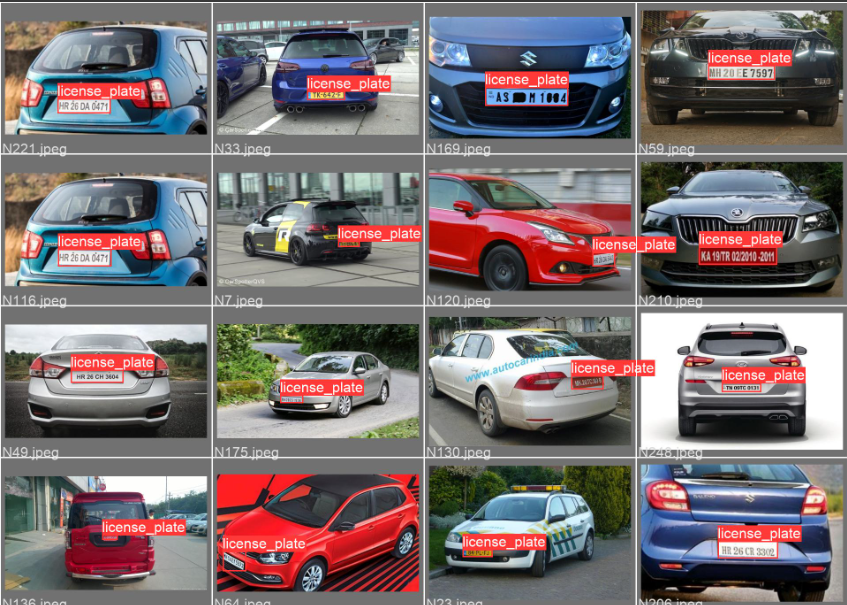
\includegraphics[width = 10cm]{img/img/Screenshot 2024-11-21 201025.png}
$
Hãy thực hiện một số thiết lập hình ảnh, điều này rất quan trọng trong việc xây dựng mô hình. Cài đặt đầu vào chúng ta cần truyền vào là 640 x 640.
$
\begin{verbatim}
# settings
INPUT_WIDTH =  640
INPUT_HEIGHT = 640    
\end{verbatim}

Hãy để tôi tải hình ảnh TEST đầu tiên, nó sẽ có một biển số xe trên đó.
\begin{verbatim}
# LOAD THE IMAGE
img = io.imread('yolov5/data_images/train/N98.jpeg')

fig = px.imshow(img)
fig.update_layout(width=700, height=400, margin=dict(l=10, r=10, b=10, t=10))
fig.update_xaxes(showticklabels=False).update_yaxes(showticklabels=False)
fig.show()
\end{verbatim}
Bây giờ, chúng ta sẽ tải mô hình YOLO của mình.
\begin{verbatim}
# LOAD YOLO MODEL
net = cv2.dnn.readNetFromONNX('./yolov5/runs/train/Model/weights/best.onnx')
net.setPreferableBackend(cv2.dnn.DNN_BACKEND_OPENCV)
net.setPreferableTarget(cv2.dnn.DNN_TARGET_CPU)
\end{verbatim}
$
Bước tiếp theo, tôi cần phân tích hình ảnh này để đưa vào mô hình YOLO và nhận kết quả dự đoán. Quan trọng - kích thước đầu vào cần được thiết lập là độ rộng 640 và chiều cao 640.
\\
Chúng ta có 25200 hàng và 6 cột. Bốn cột đầu tiên sẽ cung cấp thông tin về hộp giới hạn, bao gồm Center X, Center Y, W và H. Các giá trị này được chuẩn hóa thành 640 x 640. Hai giá trị tiếp theo là confidence và probability. Confidence cho biết độ tin cậy trong việc phát hiện hộp giới hạn, còn giá trị tiếp theo là điểm số xác suất của lớp, vì chúng ta chỉ có một lớp duy nhất là biển số xe.
\\
Hãy tạo một danh sách các hộp và độ tin cậy, và sắp xếp chúng theo thứ tự. Đồng thời, chúng ta cần xác định X_factor và Y_factor của hình ảnh.
\\
Chúng ta phải lọc các phát hiện dựa trên điểm số confidence và probability. Tôi sẽ chọn confidence > 0.4 và lọc từ class > 0.25.
\\
Một trong những vấn đề chính với mô hình YOLO là nó có thể đưa ra các hộp trùng lặp, vì cùng một đối tượng có thể được phát hiện với nhiều hộp khác nhau. Để xử lý vấn đề này, chúng ta cần thực hiện non-maximum suppression (NMS). Để làm được điều này, chúng ta cần cung cấp tất cả các hộp đã được làm sạch và các độ tin cậy của chúng.
\\
Cuối cùng, trong phần mã đó, tôi sẽ lấy các hộp giới hạn và vẽ hộp chữ nhật lên hình ảnh. Tất cả những điều này sẽ được viết thành các hàm.
$
\begin{verbatim}
def get_detections(img,net):
    # 1.CONVERT IMAGE TO YOLO FORMAT
    image = img.copy()
    row, col, d = image.shape

    max_rc = max(row,col)
    input_image = np.zeros((max_rc,max_rc,3),dtype=np.uint8)
    input_image[0:row,0:col] = image

    # 2. GET PREDICTION FROM YOLO MODEL
    blob = cv2.dnn.blobFromImage(input_image,1/255,(INPUT_WIDTH,INPUT_HEIGHT),swapRB=True,crop=False)
    net.setInput(blob)
    preds = net.forward()
    detections = preds[0]

    return input_image, detections

def non_maximum_supression(input_image,detections):

    # 3. FILTER DETECTIONS BASED ON CONFIDENCE AND PROBABILIY SCORE

    # center x, center y, w , h, conf, proba
    boxes = []
    confidences = []

    image_w, image_h = input_image.shape[:2]
    x_factor = image_w/INPUT_WIDTH
    y_factor = image_h/INPUT_HEIGHT

    for i in range(len(detections)):
        row = detections[i]
        confidence = row[4] # confidence of detecting license plate
        if confidence > 0.4:
            class_score = row[5] # probability score of license plate
            if class_score > 0.25:
                cx, cy , w, h = row[0:4]

                left = int((cx - 0.5*w)*x_factor)
                top = int((cy-0.5*h)*y_factor)
                width = int(w*x_factor)
                height = int(h*y_factor)
                box = np.array([left,top,width,height])

                confidences.append(confidence)
                boxes.append(box)

    # 4.1 CLEAN
    boxes_np = np.array(boxes).tolist()
    confidences_np = np.array(confidences).tolist()

    # 4.2 NMS
    index = cv2.dnn.NMSBoxes(boxes_np,confidences_np,0.25,0.45)

    return boxes_np, confidences_np, index

def drawings(image,boxes_np,confidences_np,index):
    # 5. Drawings
    for ind in index:
        x,y,w,h =  boxes_np[ind]
        bb_conf = confidences_np[ind]
        conf_text = 'plate: {:.0f}%'.format(bb_conf*100)

        license_text = extract_text(image,boxes_np[ind])
        # print("Plate is:" + license_text)

        cv2.rectangle(image,(x,y),(x+w,y+h),(255,0,255),2)
        cv2.rectangle(image,(x,y-30),(x+w,y),(255,0,255),-1)
        cv2.rectangle(image,(x,y+h),(x+w,y+h+25),(0,0,0),-1)

        cv2.putText(image,conf_text,(x,y-10),cv2.FONT_HERSHEY_SIMPLEX,0.7,(255,255,255),1)
        cv2.putText(image,license_text,(x,y+h+27),cv2.FONT_HERSHEY_SIMPLEX,0.7,(0,255,0),1)

    return image
\end{verbatim}

\begin{verbatim}
# predictions flow with return result
def yolo_predictions(img,net):
    # step-1: detections
    input_image, detections = get_detections(img,net)
    # step-2: NMS
    boxes_np, confidences_np, index = non_maximum_supression(input_image, detections)
    # step-3: Drawings
    result_img = drawings(img,boxes_np,confidences_np,index)
    return result_img
\end{verbatim}

\begin{verbatim}
# extrating text
def extract_text(image,bbox):
    x,y,w,h = bbox
    roi = image[y:y+h, x:x+w]

    if 0 in roi.shape:
        return 'no number'

    else:
        text = pt.image_to_string(roi)
        print(text)
        text = text.strip()

        return text

\end{verbatim}

\begin{verbatim}
import cv2
img = cv2.imread('yolov5/data_images/test/N92.jpeg')
results = yolo_predictions(img,net)
\end{verbatim}

\begin{verbatim}
# test
img = io.imread('yolov5/data_images/test/N98.jpeg')
results = yolo_predictions(img,net)
\end{verbatim}

\begin{verbatim}
pt1 =(xmin,ymin)
pt2 =(xmax,ymax)
cv2.rectangle(img,pt1,pt2,(0,255,0),3)
fig = px.imshow(img)
fig.update_layout(width=700, height=500, margin=dict(l=10, r=10, b=10, t=10))
\end{verbatim}

\begin{verbatim}
fig = px.imshow(img)
fig.update_layout(width=700, height=400, margin=dict(l=10, r=10, b=10, t=10))
fig.update_xaxes(showticklabels=False).update_yaxes(showticklabels=False)
fig.show()
\end{verbatim}

Nhấp đúp (hoặc nhấn Enter) để chỉnh sửa.
\begin{verbatim}
from google.colab.patches import cv2_imshow
import cv2

cap = cv2.VideoCapture('TEST/TEST.mp4')

nFrame = 10 # Show nFrame only
cFrame = 0
while cap.isOpened():
    ret, frame = cap.read()

    if ret == False:
        print('Unable to read video')
        break

    results = yolo_predictions(frame,net)

    # cv2.namedWindow('YOLO',cv2.WINDOW_KEEPRATIO)
    cv2_imshow(results)
    if cv2.waitKey(1) == 27 :
        break
    cFrame = cFrame+1
    if (cFrame > nFrame):
        break
cv2.destroyAllWindows()
cap.release()
\end{verbatim}
\subsection{Dự đoán kết quả từ YOLO}
Hãy thực hiện một số thiết lập hình ảnh, điều này rất quan trọng trong việc xây dựng mô hình. Cài đặt đầu vào chúng ta cần truyền vào là 640 x 640.
\begin{verbatim}
# settings
INPUT_WIDTH =  640
INPUT_HEIGHT = 640    
\end{verbatim}

Hãy để tôi tải hình ảnh TEST đầu tiên, nó sẽ có một biển số xe trên đó.
\begin{verbatim}
# LOAD THE IMAGE
img = io.imread('yolov5/data_images/train/N98.jpeg')

fig = px.imshow(img)
fig.update_layout(width=700, height=400, margin=dict(l=10, r=10, b=10, t=10))
fig.update_xaxes(showticklabels=False).update_yaxes(showticklabels=False)
fig.show()
\end{verbatim}
Bây giờ, chúng ta sẽ tải mô hình YOLO của mình.
\begin{verbatim}
# LOAD YOLO MODEL
net = cv2.dnn.readNetFromONNX('./yolov5/runs/train/Model/weights/best.onnx')
net.setPreferableBackend(cv2.dnn.DNN_BACKEND_OPENCV)
net.setPreferableTarget(cv2.dnn.DNN_TARGET_CPU)
\end{verbatim}
$
Bước tiếp theo, tôi cần phân tích hình ảnh này để đưa vào mô hình YOLO và nhận kết quả dự đoán. Quan trọng - kích thước đầu vào cần được thiết lập là độ rộng 640 và chiều cao 640.
\\
Chúng ta có 25200 hàng và 6 cột. Bốn cột đầu tiên sẽ cung cấp thông tin về hộp giới hạn, bao gồm Center X, Center Y, W và H. Các giá trị này được chuẩn hóa thành 640 x 640. Hai giá trị tiếp theo là confidence và probability. Confidence cho biết độ tin cậy trong việc phát hiện hộp giới hạn, còn giá trị tiếp theo là điểm số xác suất của lớp, vì chúng ta chỉ có một lớp duy nhất là biển số xe.
\\
Hãy tạo một danh sách các hộp và độ tin cậy, và sắp xếp chúng theo thứ tự. Đồng thời, chúng ta cần xác định X_factor và Y_factor của hình ảnh.
\\
Chúng ta phải lọc các phát hiện dựa trên điểm số confidence và probability. Tôi sẽ chọn confidence > 0.4 và lọc từ class > 0.25.
\\
Một trong những vấn đề chính với mô hình YOLO là nó có thể đưa ra các hộp trùng lặp, vì cùng một đối tượng có thể được phát hiện với nhiều hộp khác nhau. Để xử lý vấn đề này, chúng ta cần thực hiện non-maximum suppression (NMS). Để làm được điều này, chúng ta cần cung cấp tất cả các hộp đã được làm sạch và các độ tin cậy của chúng.
\\
Cuối cùng, trong phần mã đó, tôi sẽ lấy các hộp giới hạn và vẽ hộp chữ nhật lên hình ảnh. Tất cả những điều này sẽ được viết thành các hàm.
$
\begin{verbatim}
def get_detections(img,net):
    # 1.CONVERT IMAGE TO YOLO FORMAT
    image = img.copy()
    row, col, d = image.shape

    max_rc = max(row,col)
    input_image = np.zeros((max_rc,max_rc,3),dtype=np.uint8)
    input_image[0:row,0:col] = image

    # 2. GET PREDICTION FROM YOLO MODEL
    blob = cv2.dnn.blobFromImage(input_image,1/255,(INPUT_WIDTH,INPUT_HEIGHT),swapRB=True,crop=False)
    net.setInput(blob)
    preds = net.forward()
    detections = preds[0]

    return input_image, detections

def non_maximum_supression(input_image,detections):

    # 3. FILTER DETECTIONS BASED ON CONFIDENCE AND PROBABILIY SCORE

    # center x, center y, w , h, conf, proba
    boxes = []
    confidences = []

    image_w, image_h = input_image.shape[:2]
    x_factor = image_w/INPUT_WIDTH
    y_factor = image_h/INPUT_HEIGHT

    for i in range(len(detections)):
        row = detections[i]
        confidence = row[4] # confidence of detecting license plate
        if confidence > 0.4:
            class_score = row[5] # probability score of license plate
            if class_score > 0.25:
                cx, cy , w, h = row[0:4]

                left = int((cx - 0.5*w)*x_factor)
                top = int((cy-0.5*h)*y_factor)
                width = int(w*x_factor)
                height = int(h*y_factor)
                box = np.array([left,top,width,height])

                confidences.append(confidence)
                boxes.append(box)
\end{verbatim}
\begin{verbatim}
    # 4.1 CLEAN
    boxes_np = np.array(boxes).tolist()
    confidences_np = np.array(confidences).tolist()

    # 4.2 NMS
    index = cv2.dnn.NMSBoxes(boxes_np,confidences_np,0.25,0.45)

    return boxes_np, confidences_np, index

def drawings(image,boxes_np,confidences_np,index):
    # 5. Drawings
    for ind in index:
        x,y,w,h =  boxes_np[ind]
        bb_conf = confidences_np[ind]
        conf_text = 'plate: {:.0f}%'.format(bb_conf*100)

        license_text = extract_text(image,boxes_np[ind])
        # print("Plate is:" + license_text)

        cv2.rectangle(image,(x,y),(x+w,y+h),(255,0,255),2)
        cv2.rectangle(image,(x,y-30),(x+w,y),(255,0,255),-1)
        cv2.rectangle(image,(x,y+h),(x+w,y+h+25),(0,0,0),-1)

        cv2.putText(image,conf_text,(x,y-10),cv2.FONT_HERSHEY_SIMPLEX,0.7,(255,255,255),1)
        cv2.putText(image,license_text,(x,y+h+27),cv2.FONT_HERSHEY_SIMPLEX,0.7,(0,255,0),1)

    return image
\end{verbatim}

\begin{verbatim}
# predictions flow with return result
def yolo_predictions(img,net):
    # step-1: detections
    input_image, detections = get_detections(img,net)
    # step-2: NMS
    boxes_np, confidences_np, index = non_maximum_supression(input_image, detections)
    # step-3: Drawings
    result_img = drawings(img,boxes_np,confidences_np,index)
    return result_img
\end{verbatim}

\begin{verbatim}
# extrating text
def extract_text(image,bbox):
    x,y,w,h = bbox
    roi = image[y:y+h, x:x+w]

    if 0 in roi.shape:
        return 'no number'

    else:
        text = pt.image_to_string(roi)
        print(text)
        text = text.strip()

        return text

\end{verbatim}

\begin{verbatim}
import cv2
img = cv2.imread('yolov5/data_images/test/N92.jpeg')
results = yolo_predictions(img,net)
\end{verbatim}

\begin{verbatim}
# test
img = io.imread('yolov5/data_images/test/N98.jpeg')
results = yolo_predictions(img,net)
\end{verbatim}

\begin{verbatim}
pt1 =(xmin,ymin)
pt2 =(xmax,ymax)
cv2.rectangle(img,pt1,pt2,(0,255,0),3)
fig = px.imshow(img)
fig.update_layout(width=700, height=500, margin=dict(l=10, r=10, b=10, t=10))
\end{verbatim}

\begin{verbatim}
fig = px.imshow(img)
fig.update_layout(width=700, height=400, margin=dict(l=10, r=10, b=10, t=10))
fig.update_xaxes(showticklabels=False).update_yaxes(showticklabels=False)
fig.show()
\end{verbatim}

Nhấp đúp (hoặc nhấn Enter) để chỉnh sửa.
\begin{verbatim}
from google.colab.patches import cv2_imshow
import cv2

cap = cv2.VideoCapture('TEST/TEST.mp4')

nFrame = 10 # Show nFrame only
cFrame = 0
while cap.isOpened():
    ret, frame = cap.read()

    if ret == False:
        print('Unable to read video')
        break

    results = yolo_predictions(frame,net)

    # cv2.namedWindow('YOLO',cv2.WINDOW_KEEPRATIO)
    cv2_imshow(results)
    if cv2.waitKey(1) == 27 :
        break
    cFrame = cFrame+1
    if (cFrame > nFrame):
        break
cv2.destroyAllWindows()
cap.release()
\end{verbatim}

%9
\section{Kết luận}
Với sự gia tăng số lượng phương tiện, việc theo dõi phương tiện đã trở thành một lĩnh vực nghiên cứu quan trọng để kiểm soát giao thông hiệu quả, giám sát và tìm kiếm xe bị đánh cắp. Để đạt được mục đích này, việc phát hiện và nhận dạng biển số xe trong thời gian thực là rất quan trọng. Do sự biến đổi về nền tảng, màu sắc và kiểu chữ, kích thước biển số, và các ký tự không chuẩn, việc nhận dạng biển số xe là một thách thức lớn ở các quốc gia đang phát triển. Để khắc phục các vấn đề này, nghiên cứu này áp dụng chiến lược học sâu để cải thiện hiệu quả nhận dạng biển số xe. Các hình ảnh thu thập được đã được chụp dưới các điều kiện ánh sáng/độ tương phản khác nhau, khoảng cách từ camera, góc quay thay đổi, và đã được xác nhận để đạt được tỷ lệ nhận dạng cao. Phương pháp này có thể được sử dụng hiệu quả bởi các cơ quan thực thi pháp luật và các tổ chức tư nhân để cải thiện an ninh quốc gia. Công việc trong tương lai có thể bao gồm việc huấn luyện và xác nhận thuật toán hiện có bằng phương pháp phân loại lai và cải thiện độ bền của hệ thống nhận dạng biển số xe trong các điều kiện thời tiết khác nhau.
\\
Tất cả các tệp bạn cũng có thể tìm thấy trên trang của tôi.\href{https://github.com/Asikpalysik/Automatic-License-Plate-Detection}{GITHUB} 
Nếu bạn thấy bài viết này hữu ích, vui lòng đánh giá cao (UPVOTE), và nếu bạn có bất kỳ câu hỏi nào, đừng ngần ngại hỏi.
\href{http://aslanahmedov.com.}{Liên hệ với tôi.}
\newline
\\
----------------------------------------------------------------------------------------------------------------------------------------------------------\\
\textbf{BÁO CÁO LÀM VIỆC HÀNG TUẦN}
\begin{itemize}
    \item \textbf{(a) Ngày họp}: chủ nhật hàng tuần.
    \item \textbf{(b) Thành viên tham dự}: tất cả thành viên.
    \item \textbf{(c) Phân công}:
        \begin{itemize}
            \item Thạch,Phát,Huy: viết latex(trong 1 tuần)
            \item Kiên,Đăng: powerpoint(trong 1 tuần)
            \item Tài: source code(2 tuần)
        \end{itemize}
    \item \textbf{(d) Tiến độ làm các tuần}:
        \begin{itemize}
            \item tuần 1:
                \begin{itemize}
                    \item Nội dung phân công: tìm hiểu Github và google colab.
                    \item Người được phân công: cả nhóm.
                    \item Tiến độ làm: hoàn thành.
                    \item Công việc đã làm: tìm hiểu Github và Google colab.
                    \item Công việc chưa làm: Phân chia công việc project.
                \end{itemize}
            \item tuần 2:
                \begin{itemize}
                    \item Nội dung phân công: làm latex, powerpoint,source code, quay video.
                    \item Người được phân công:
                        \begin{itemize}
                            \item Thạch, Huy, Phát: Latex.
                            \item Đăng, Kiên: powerpoint.
                            \item Tài: source code, quay video.
                        \end{itemize}
                    \item Tiến độ làm: 70\% công việc.
                    \item Công việc đã làm: Latex, powerpoint.
                    \item Công việc chưa làm: video, quay video .
                \end{itemize}
            \item Tuần 3:
               \begin{itemize}
                    \item Nội dung phân công: source code, quay video.
                    \item Người được phân công:
                        \begin{itemize}
                            \item cả nhóm làm video và source code
                        \end{itemize}
                    \item Tiến độ làm: 70\% công việc.
                    \item Công việc đã làm: Latex, powerpoint.
                    \item Công việc chưa làm: video, quay video .
                \end{itemize}
            \item Tuần 4:
                \begin{itemize}
                    \item Nội dung phân công: source code, quay video.
                    \item Người được phân công:
                        \begin{itemize}
                            \item cả nhóm làm video và source code
                        \end{itemize}
                    \item Tiến độ làm: 100\% công việc.
                    \item Công việc đã làm: Latex, powerpoint, source code, quay video.
                    \item Công việc chưa làm: hết .
                \end{itemize}
        \end{itemize}
        
\end{itemize}
\end{document}
